\documentclass[12pt]{article}
\usepackage[margin=1in]{geometry}
\usepackage{fancyhdr}
\usepackage[T1]{fontenc} % Some font fixes
\usepackage{amsmath, amssymb, amsthm} % Allows extra math commands
\usepackage{listings}
\usepackage{xcolor}
\usepackage{graphicx}
\usepackage[hidelinks]{hyperref} % Removes colored borders around links
\usepackage{titlesec}
\usepackage{tocloft} % For table of contents formatting

% Header and Footer
\pagestyle{fancy}
\fancyhf{} % Clears existing header and footer settings
\fancyhead[L]{ASHISH KOSANA} % Left part of header (name)
\fancyhead[R]{\thepage} % Right part of header (page number)

% Define colors for code
\definecolor{backcolour}{rgb}{0.92,0.92,0.90} % Light gray background
\definecolor{Green}{rgb}{0,0.6,0}            % Green for comments
\definecolor{Blue}{rgb}{0,0,1}               % Blue for keywords
\definecolor{Maroon}{rgb}{0.58,0,0.82}       % Maroon for strings

% Formatting style for C++ code
\lstdefinestyle{cppcode}{
    language=C++,                    % Set language to C++
    basicstyle=\ttfamily,            % Monospaced font (ttfamily)
    commentstyle=\color{Green},      % Green for comments
    keywordstyle=\color{Blue},       % Blue for keywords
    stringstyle=\color{Maroon},      % Maroon for strings
    tabsize=4,                       % Set tab size to 4 spaces
    columns=flexible,                % Flexible column alignment
    keepspaces=true,                 % Preserve spaces in code
    numbers=left,                    % Show line numbers on the left
    numberstyle=\tiny,               % Smaller font size for line numbers
    showstringspaces=false,          % Do not show spaces in strings
    backgroundcolor=\color{backcolour}, % Light gray background color
    frame=single,                    % Add a border around the code block
    breaklines=true                  % Break long lines in the code block
}

% Formatting style for Makefile code (different from C++)
\lstdefinestyle{makefile}{
    language=[gnu]make,              % Set language to GNU Makefile syntax
    basicstyle=\ttfamily,            % Monospaced font (ttfamily)
    keywordstyle=\color{Blue},       % Blue for keywords like `all`, `clean`, etc.
    stringstyle=\color{Maroon},      % Maroon for strings (if any)
    commentstyle=\color{Green},      % Green for comments in Makefiles (# comments)
    tabsize=4,                       % Set tab size to 4 spaces
    numbers=left,                    % Show line numbers on the left
    numberstyle=\tiny,               % Smaller font size for line numbers
    showstringspaces=false,          % Do not show spaces in strings
    backgroundcolor=\color{backcolour}, % Light gray background color
    frame=single,                    % Add a border around the code block
    breaklines=true                  % Break long lines in the code block
}

% Title Formatting
\titleformat{\section}{\large\bfseries}{\thesection}{1em}{}
\titleformat{\subsection}{\normalsize\bfseries}{\thesubsection}{1em}{}

% Set TOC depth to include all levels
\setcounter{tocdepth}{3}

% Document Starts
\begin{document}

% First Page
\begin{center}
\thispagestyle{empty}
\noindent
\textbf{\Large COMPUTING IV Sec 202:Project Portfolio} \\[1em]
\textbf{\Large Ashish Kosana} \\[1em]
\textbf{\Large Fall 2024}

\vspace{1cm}  % Reduced space
\end{center}

    \tableofcontents
    
    \vspace{1cm}  % Space before "Time to Complete"
    \textbf{\Large Time to Complete: 13 Hours}


% Set up headers for subsequent pages
\clearpage
\pagestyle{fancy}
\fancyhf{}
\fancyhead[L]{ASHISH KOSANA}
\fancyhead[R]{\thepage}

% Set up headers for subsequent pages
\clearpage
\pagestyle{fancy}
\fancyhf{}
\fancyhead[L]{ASHISH KOSANA}
\fancyhead[R]{\thepage}

% PS0: Hello SFML
\section{PS0: Hello SFML}
\subsection{Overview}
I have made a simple program using SFML that shows a moving sprite  and a rectangle on the sfml window. The sprite moves when I press keyboard keys, and the background color changes to four different colors for four different keys in the keyboard. This project helped me understand how to create basic graphics and handle user input.

\subsection{What I Accomplished}
1. I have created a program where the sprite moves smoothly and responds to key presses.
\newline
2. I have implemented the sprite movement using delta time calculations, where the sprite moves different sides for different keys.
\newline
3. I have added  background colour changing feature such that it creates fun for the user.

\subsection{What I Learned}
1. I have learned how to create a window using sfml and load shapes and sprites into it.
\newline
2.  I have understood how to detect key presses and make the program respond to them.
\newline
3.  I have learned how to implement graphics in c++ using sfml

\subsection{Discussion of Key Algorithms \& Data structures}
1. \textbf{Data structures:}
\newline
==$>$  sf::Sprite for the image that moves.
\newline
==$>$  sf::RectangleShape for a rectangle that stays on the screen.
\newline
==$>$  sf::Vector2f to handle positions and movement.
\newline
==$>$  sf::Clock and sf::Time to measure time and control movement.
\newline
2. \textbf{Key Algorithms:}
\newline
==$>$  Movement: The sprite moves in different directions when I press W, A, S, D, or the arrow keys.
\newline
==$>$  Delta Time: I have used time to make sure the sprite moves smoothly and with the same speed.
\newline
==$>$  Color Change: The background color changes depending on which key is pressed.
\newline
==$>$prite Movement:Ensure smooth movement using a frame rate-independent formula:
distance=movementSpeed×deltaTime.
\newline
\textbf{Object Oriented Designs:}
\newline
==$>$Abstraction:
\newline
I have used  abstractions to focus on implementing higher-level functionality like controlling the sprite’s movement and changing the background color. 
\newline
==$>$Interaction between objects:
\newline
I have learned that objects can interact with each other. For example, sf::RenderWindow interacts with sf::Sprite to display the sprite, while sf::Keyboard interacts with sf::Sprite to move it
\subsection{What I Already Knew}
==$>$I am familier with c++ language.
\subsection{Challenges}
==$>$Learning how to use SFML for the first time, such as creating a window, drawing shapes, and loading images, was a bit challenging.
\newline
==$>$As i was learning sfml for the first time Combining graphics programming with C++ was tricky.
\subsection{Codes}

\subsubsection{Makefile}

\begin{lstlisting}[style=cppcode]
CC = g++
CFLAGS = --std=c++20 -Wall -Werror -pedantic -g
LIB = -lsfml-graphics -lsfml-audio -lsfml-window -lsfml-system
DEPS = 
OBJECTS = main.o
PROGRAM = sfml-app

.PHONY: all clean lint

all: $(PROGRAM)

%.o: %.cpp $(DEPS)
    $(CC) $(CFLAGS) -c $<

$(PROGRAM): main.o $(OBJECTS)
    $(CC) $(CFLAGS) -o $@ $^ $(LIB)

clean:
    rm *.o $(PROGRAM)

lint:
    cpplint *.cpp *.hpp
\end{lstlisting}

\subsubsection{main.cpp}
\begin{lstlisting}[style=cppcode]
#include<iostream>
#include <SFML/Graphics.hpp>
int main() {
    sf::RenderWindow window(sf::VideoMode(1000, 800), "Ashish's Moving Sprite");
    sf::RectangleShape rec(sf::Vector2f(100, 120));
    rec.setFillColor(sf::Color::Red);
    rec.setPosition(50.f, 55.f);
    window.setFramerateLimit(60);
    sf::Texture spriteTexture;
    if (!spriteTexture.loadFromFile("Sprite.png")) {
        std::cerr << "image loading failed!" << std::endl;
        return -1;
    }
    sf::Sprite sprite;
    sprite.setTexture(spriteTexture);
    sprite.setScale(0.5f, 0.5f);
    sf::Vector2u windowSize = window.getSize();
    sf::FloatRect spriteBounds = sprite.getGlobalBounds();
    float posX = (windowSize.x - spriteBounds.width) / 3.0f;
    float posY = (windowSize.y - spriteBounds.height) / -20.0f;
    sprite.setPosition(posX, posY);
    sprite.setScale(0.2f, 0.2f);
    float movementSpeed = 200.0f;
    sf::Clock frameClock;
    sf::Color backgroundColor = sf::Color::White;
    while (window.isOpen()) {
        sf::Event event;
        while (window.pollEvent(event)) {
            if(event.type == sf::Event::Closed) {
                window.close();
            }
        }
        sf::Time elapsedTime = frameClock.restart();
        float deltaTime = elapsedTime.asSeconds();
        backgroundColor = sf::Color::White;
        if (sf::Keyboard::isKeyPressed(sf::Keyboard::Left) ||
            sf::Keyboard::isKeyPressed(sf::Keyboard::A)) {
            sprite.move(-movementSpeed * deltaTime, 0);
            backgroundColor = sf::Color::Magenta;
        }
        if (sf::Keyboard::isKeyPressed(sf::Keyboard::Right) ||
            sf::Keyboard::isKeyPressed(sf::Keyboard::D)) {
            sprite.move(movementSpeed * deltaTime, 0);
            backgroundColor = sf::Color::Green;
        }
        if (sf::Keyboard::isKeyPressed(sf::Keyboard::Up) ||
            sf::Keyboard::isKeyPressed(sf::Keyboard::W)) {
            sprite.move(0, -movementSpeed * deltaTime);
            backgroundColor = sf::Color::Cyan;
        }
        if (sf::Keyboard::isKeyPressed(sf::Keyboard::Down) ||
            sf::Keyboard::isKeyPressed(sf::Keyboard::S)) {
            sprite.move(0, movementSpeed * deltaTime);
            backgroundColor = sf::Color::Yellow;
        }
        window.clear(backgroundColor);
        window.draw(sprite);
        window.draw(rec);
        window.display();
    }
    return 0;
}
\end{lstlisting}

\subsubsection{screenshot}
\begin{figure}[tbh]
	\centering
	
\includegraphics[width=10cm]{comp 4/images/ps0_screenshot.png}
	\caption{My sfml window}
	
\end{figure}

\newpage

% PS1a \& ps1b: LFSR \& PhotoMagic
\section{PS1: LFSR \& PhotoMagic}
\subsection{Overview}
In this project, I have implemented a Fibonacci Linear Feedback Shift Register (LFSR) that simulates pseudo-random bit generation. This LFSR uses specific tap positions to calculate new bits using XOR operations.  
\newline
I have Extended the use of the LFSR to encrypt and decrypt images by changing the pixel values using the pseudo-random sequence generated by the LFSR.
\newline
==$>$The encryption process uses the pseudo-random bit sequence generated by the LFSR to alter the red, green, and blue (RGB) values of each pixel in the input image.
\newline
==$>$The Decryption process also uses the same LFSR configuration to regenerate the identical pseudo-random sequence used in encryption process.

\subsection{What I Accomplished}
 1. I have implemented FibLFSR class for simulating the behaviour of LFSR.
\newline
2. I have implemented the step function which which moves the bit position one to left and adds new bit.
\newline
3. I have successfully implemented encryption and decryption for images using LFSR.
\newline
4. I have ensured that the decrypted image matches the original image.
\subsection{What I Learned}
==$>$ I have learned that an LFSR works by shifting the bits to the left and replacing the empty bit with the result of XORing specific tap bits.
\newline
==$>$I have learned how to write and run unit tests using the Boost framework
\newline
==$>$I have understood LFSR and how it generates pseudo-random sequences.
\newline
==$>$I have learned that how to change the image pixel values using C++ and SFML.
\subsection{Discussion of Key Algorithms}
\textbf{1.Data structures:}
\newline
i.) std::string:
\newline
==$>$I have used a string to represent the LFSR state. Each character in the string represents a bit either '0' or '1'.
\newline
ii.) sf::Image:
\newline 
==$>$To handle the input and output images.
\newline
iii.)std::vector: 
\newline
==$>$For processing pixel data.
\newline
\textbf{2.Algorithms:}
\newline
1. Step Function (step()):
\newline
==$>$ It calculates the new bit by XORing the leftmost bit with the bits at the tap positions.
\newline
2.Image Encryption: 
\newline
==$>$Pixel values were altered by performing XOR operations between pixel data and LFSR output.
\subsection{What I Already Knew}
==$>$ I know basic XOR operations.
\newline
==$>$Basic C++ syntax, including classes, constructors, and functions.
\newline
\textbf{Object Oriented Designs:}
\newline
==$>$Classes and Objects: FibLFSR is the main class, and objects of this class are created to represent LFSRs.
\newline
==$>$Abstraction: The FibLFSR class abstracts the LFSR functionality.
\subsection{Challenges}
==$>$For the first time i have faced difficulty in understanding the FIBLFSR algorithm.
\newline
==$>$I have faced difficulty in Encrypting and Decrypting the image using the 16 bit seed.
\newline
==$>$I felt little bit difficult in xor'ing the pixels.


\subsection{Codes}

\subsubsection{Makefile}
\begin{lstlisting}[style=cppcode]
CXX = g++
CXXFLAGS = -std=c++11 -Wall -Wextra -Werror -pedantic
SFML_LIBS = -lsfml-graphics -lsfml-window -lsfml-system
BOOST_LIBS = -lboost_unit_test_framework
AR = ar
ARFLAGS = rcs

all: PhotoMagic test PhotoMagic.a

PhotoMagic: main.o PhotoMagic.o FibLFSR.o
	$(CXX) $(CXXFLAGS) -o $@ $^ $(SFML_LIBS)

test: test.o FibLFSR.o PhotoMagic.o
	$(CXX) $(CXXFLAGS) -o $@ $^ $(SFML_LIBS) $(BOOST_LIBS)

PhotoMagic.a: PhotoMagic.o FibLFSR.o
	$(AR) $(ARFLAGS) $@ $^

%.o: %.cpp
	$(CXX) $(CXXFLAGS) -c $< -o $@

clean:
	rm -f *.o PhotoMagic test PhotoMagic.a

.PHONY: all clean
\end{lstlisting}
\subsubsection{main.cpp}
\begin{lstlisting}[style=cppcode]

// CopyRight 2024 Ashish kosana
#include <iostream>
#include <bitset>
#include "PhotoMagic.hpp"
#include "FibLFSR.hpp"
#include <SFML/Graphics.hpp>

// Converts alphanumeric key to a binary seed
std::string convertKeyToBinary(const std::string &key) {
    std::string binarySeed;
    for (char c : key) {
        binarySeed += std::bitset<8>(c).to_string();
    }
    // Ensure the binary seed is exactly 16 bits long
    if (binarySeed.size() > 16) {
        binarySeed = binarySeed.substr(0, 16);
    } else if (binarySeed.size() < 16) {
        binarySeed.append(16 - binarySeed.size(), '0');
    }
    return binarySeed;
}

int main(int argc, char* argv[]) {
    if (argc != 4) {
        std::cerr << "Usage: " << argv[0]
                  << " <input-file> <output-file> <LFSR-seed>" << std::endl;
        return 1;
    }

    std::string inputFile = argv[1];
    std::string outputFile = argv[2];
    std::string seed = argv[3];

    // Convert the alphanumeric seed to binary
    std::string binarySeed = convertKeyToBinary(seed);

    sf::Image inputImage;
    if (!inputImage.loadFromFile(inputFile)) {
        std::cerr << "Failed to load input image." << std::endl;
        return 1;
    }

    PhotoMagic::FibLFSR lfsr(binarySeed);
    sf::Image outputImage = inputImage;
    PhotoMagic::transform(outputImage, &lfsr);

    if (!outputImage.saveToFile(outputFile)) {
        std::cerr << "Failed to save output image." << std::endl;
        return 1;
    }

    sf::Texture inputTexture, outputTexture;
    inputTexture.loadFromImage(inputImage);
    outputTexture.loadFromImage(outputImage);

    sf::Sprite inputSprite(inputTexture), outputSprite(outputTexture);

    sf::Vector2u size = inputImage.getSize();
    sf::RenderWindow inputWindow(sf::VideoMode(size.x, size.y), "Original Image");
    sf::RenderWindow outputWindow(sf::VideoMode(size.x, size.y), "Transformed Image");

    while (inputWindow.isOpen() && outputWindow.isOpen()) {
        sf::Event event;
        while (inputWindow.pollEvent(event)) {
            if (event.type == sf::Event::Closed)
                inputWindow.close();
        }
        while (outputWindow.pollEvent(event)) {
            if (event.type == sf::Event::Closed)
                outputWindow.close();
        }

        inputWindow.clear();
        inputWindow.draw(inputSprite);
        inputWindow.display();

        outputWindow.clear();
        outputWindow.draw(outputSprite);
        outputWindow.display();
    }
    return 0;
}

\end{lstlisting}
\subsubsection{FibLFSR.hpp}
\begin{lstlisting}[style=cppcode]
// CopyRight 2024 Ashish kosana
#ifndef FIBLFSR_HPP
#define FIBLFSR_HPP

#include <string>
#include <iostream>

namespace PhotoMagic {

class FibLFSR {
 public:
explicit FibLFSR(std::string seed);
    int step();
    int generate(int k);
    std::string toString() const;

    friend std::ostream& operator<<(std::ostream& os, const FibLFSR& lfsr);
    friend std::istream& operator>>(std::istream& is, FibLFSR& lfsr);

 private:
    std::string register_state;
};

}  // namespace PhotoMagic

#endif  // FIBLFSR_HPP
\end{lstlisting}
\subsubsection{FibLFSR.cpp}
\begin{lstlisting}[style=cppcode]
#include <stdexcept>
#include "FibLFSR.hpp"

namespace PhotoMagic {

FibLFSR::FibLFSR(std::string seed) : register_state(seed) {
    if (seed.empty() || seed.find_first_not_of("01") != std::string::npos) {
        throw std::invalid_argument("Seed must be a non-empty binary string");
    }
}

int FibLFSR::step() {
    int new_bit = (register_state[0] - '0') ^ (register_state[2] - '0') ^ 
                  (register_state[3] - '0') ^ (register_state[5] - '0');
    register_state = register_state.substr(1) + std::to_string(new_bit);
    return new_bit;
}

int FibLFSR::generate(int k) {
    int result = 0;
    for (int i = 0; i < k; ++i) {
        result = (result << 1) | step();
    }
    return result;
}

std::string FibLFSR::toString() const {
    return register_state;
}

std::ostream& operator<<(std::ostream& os, const FibLFSR& lfsr) {
    return os << lfsr.toString();
}

std::istream& operator>>(std::istream& is, FibLFSR& lfsr) {
    std::string seed;
    is >> seed;
    lfsr = FibLFSR(seed);
    return is;
}

}  // namespace PhotoMagic
\end{lstlisting}
\subsubsection{PhotoMagic.hpp}
\begin{lstlisting}[style=cppcode]
// CopyRight 2024 Ashish kosana
#ifndef PHOTOMAGIC_HPP
#define PHOTOMAGIC_HPP

#include <SFML/Graphics.hpp>
#include "FibLFSR.hpp"

namespace PhotoMagic {
void transform(sf::Image &image, FibLFSR *lfsr);
}

#endif  // PHOTOMAGIC_HPP

\end{lstlisting}
\subsubsection{PhotoMagic.cpp}
\begin{lstlisting}[style=cppcode]
// CopyRight 2024 Ashish kosana
#include "PhotoMagic.hpp"
namespace PhotoMagic {
void transform(sf::Image& image, FibLFSR* lfsr) {
        sf::Vector2u size = image.getSize();
        for (unsigned int y = 0; y < size.y; ++y) {
            for (unsigned int x = 0; x < size.x; ++x) {
                sf::Color pixel = image.getPixel(x, y);
                uint8_t r = pixel.r ^ lfsr->generate(8);
                uint8_t g = pixel.g ^ lfsr->generate(8);
                uint8_t b = pixel.b ^ lfsr->generate(8);
                image.setPixel(x, y, sf::Color(r, g, b, pixel.a));
}
}
}
}  // namespace PhotoMagic
\end{lstlisting}

\subsubsection{test.cpp}
\begin{lstlisting}[style=cppcode]
// CopyRight [2024] Ashish Kosana
#include <iostream>
#include <string>
#include <SFML/Graphics.hpp>
#include "FibLFSR.hpp"
#include "PhotoMagic.hpp"

#define BOOST_TEST_DYN_LINK
#define BOOST_TEST_MODULE PhotoMagicTest
#include <boost/test/unit_test.hpp>

using PhotoMagic::FibLFSR;
using PhotoMagic::transform;

BOOST_AUTO_TEST_CASE(testInitialization) {
    FibLFSR l("1010101010101010");
    BOOST_REQUIRE_EQUAL(l.toString(), "1010101010101010");
}

BOOST_AUTO_TEST_CASE(testEmptySeed) {
    BOOST_CHECK_THROW(FibLFSR l(""), std::invalid_argument);
}

BOOST_AUTO_TEST_CASE(testInvalidSeedCharacters) {
    BOOST_CHECK_THROW(FibLFSR l("1010A01010101010"), std::invalid_argument);
}

BOOST_AUTO_TEST_CASE(testImageTransform) {
    sf::Image image;
    if (!image.loadFromFile("input.png")) {
        BOOST_FAIL("Failed to load test image file 'input.png'");
    }

    sf::Image originalImage = image;

    // Initialize LFSR with a seed and transform the image (encrypt)
    FibLFSR lfsrEncrypt("1010101010101010");
    transform(image, &lfsrEncrypt);

    // Reinitialize LFSR with the same seed and transform the image again (decrypt)
    FibLFSR lfsrDecrypt("1010101010101010");
    transform(image, &lfsrDecrypt);

    // Verify if each pixel in the decrypted image matches the original
    sf::Vector2u size = image.getSize();
    for (unsigned int x = 0; x < size.x; ++x) {
        for (unsigned int y = 0; y < size.y; ++y) {
            BOOST_REQUIRE(image.getPixel(x, y) == originalImage.getPixel(x, y));
        }
    }
}

\end{lstlisting}
\newpage
\subsubsection{screenshot}
\begin{figure}[tbh]
	\centering
	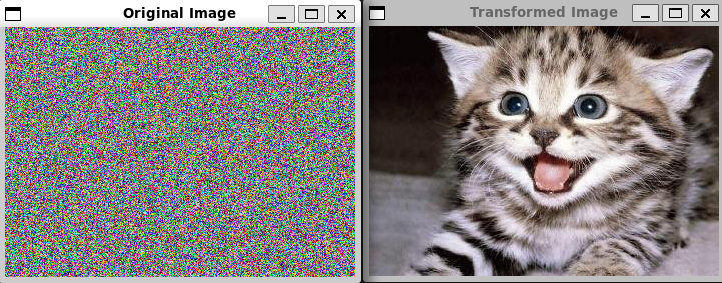
\includegraphics[width=10cm]{comp 4/images/ps1b_screenshot1 1.png}
	\caption{Encrypted Image}

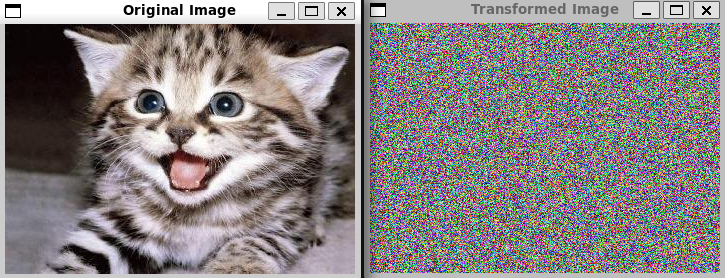
\includegraphics[width=10cm]{comp 4/images/ps1b_screenshot1 2.png}
\caption{Decrypted Image}
	
\end{figure}

\newpage
% PS1a \& Photomagic: LFSR \& PhotoMagic

\newpage
% PS2: Pentaflake
\section{PS2: Pentaflake}
\subsection{Overview}
I have created a program using SFML that generates a visual structure called the Pentaflake. This structure starts with a pentagon and adds smaller pentagons around it through a recursive process. Users can specify the size of the base pentagon and how many times to repeat this process. The Pentaflake rotates and changes colors based on its position and depth, making it visually engaging
\subsection{What I Accomplished}
==$>$I have implemented a recursive function that draws smaller pentagons around a central pentagon, creating the fractal effect.
\newline
==$>$Used SFML to create a window where the Pentaflake is displayed and updated in real-time.
\newline
==$>$I have included rotation functionality so that the entire pentaflake can spin, making it more engaging for viewers.
\subsection{What I Learned}
==$>$I have learned the concept of recursion and how it can be applied to generate complex shapes like pentagons.
\subsection{Discussion of Key Algorithms}
\textbf{Data Structures:}
\newline
1. std::vector<sf::ConvexShape>:
\newline
==$>$Used to store all the pentagons that make up the Pentaflake.
\newline
2. sf::Vector2f: 
\newline
==$>$Used for handling positions of the pentagons in 2D space.
\newline
\textbf{Algorithms:}
\newline
1. Recursive Drawing:
\newline
==$>$The createPentaflake function calls itself to draw smaller pentagons around each existing one until reaching the specified depth.
\newline
2. Rotation Logic:
\newline
==$>$The entire Pentaflake is rotated around its center using SFML's transformation functions, adding movement to the display.
\newline
\textbf{Object Oriented Designs:}
\newline
==$>$Recurssion:
\newline
The method createPentaflake calls itself to generate smaller pentagons within the main pentagon.
\newline
==$>$Inheritance:
\newline
The class Pentaflake is inherited from sf::Drawable.
\subsection{What I Already Knew}
==$>$I was familiar with C++ programming basics, including syntax and data types.
\subsection{Challenges}
==$>$I have faced challenge in writing the recurssion logic for generating the small pentagons around the base pentagon.
\newline
==$>$I have faced little difficulty while linking the sfml and boost libraries.
\newline
==$>$I have faced difficult over calculating the dynamic color for each pentagon.
\subsection{Codes}
\subsubsection{Makefile}
\begin{lstlisting}[style=cppcode]
CC = g++
CFLAGS = --std=c++20 -Wall -Werror -pedantic -g
LIB = -lsfml-graphics -lsfml-audio -lsfml-window -lsfml-system -lboost_unit_test_framework
DEPS = penta.hpp
SOURCES = penta.cpp
PROGRAM = Penta

.PHONY: all clean lint

all: $(PROGRAM)

%.o: %.cpp $(DEPS)
	$(CC) $(CFLAGS) -c $<

penta.o: penta.cpp $(DEPS)
	$(CC) $(CFLAGS) -c $<

$(PROGRAM): main.o penta.o
	$(CC) $(CFLAGS) -o $@ $^ $(LIB)

clean:
	rm -f *.o $(PROGRAM)

lint:
	cpplint *.cpp *.hpp
\end{lstlisting}
\newpage
\subsubsection{main.cpp}
\begin{lstlisting}[style=cppcode]
// copyright [2024] Ashish Kosana
#include <iostream>
#include <SFML/Graphics.hpp>
#include "penta.hpp"
int main(int argc, char* argv[]) {
if (argc != 3) {
std::cerr << "Usage: " << argv[0] <<
" <side_length> <recursion_depth>" << std::endl;
return 1;
}
double L = std::stod(argv[1]);
int N = std::stoi(argv[2]);
sf::RenderWindow window(sf::VideoMode(800, 800), "Pentaflake");
window.setFramerateLimit(60);
Pentaflake pentaflake(L, N);
while (window.isOpen()) {
sf::Event event;
while (window.pollEvent(event)) {
if (event.type == sf::Event::Closed)
window.close();
}
window.clear(sf::Color::Cyan);
window.draw(pentaflake);
window.display();
}
return 0;
}
\end{lstlisting}
\subsubsection{penta.hpp}
\begin{lstlisting}[style=cppcode]
// copyright [2024] Ashish Kosana
#pragma once
#include <cmath>
#include <SFML/Graphics.hpp>

class Pentaflake : public sf::Drawable {
 public:
    Pentaflake(double sideLength, int depth);

 private:
    void draw(sf::RenderTarget& target, sf::RenderStates states) const override;
    void createPentaflake(double sideLength, int depth, sf::Vector2f position, float rotation);

    std::vector<sf::ConvexShape> pentagons;
    const double PHI = (1 + std::sqrt(5)) / 2;
};
\end{lstlisting}
\subsubsection{penta.cpp}
\begin{lstlisting}[style=cppcode]
#include "penta.hpp"
#include <ctime>

Pentaflake::Pentaflake(double sideLength, int depth) {
    sf::Vector2f center(400, 400);
    createPentaflake(sideLength, depth, center, 0);
}

void Pentaflake::draw(sf::RenderTarget& target, sf::RenderStates states) const {
    static float rotationAngle = 0.0f;
    rotationAngle += 100.5f;  // Adjust this value to change rotation speed

    sf::Transform rotation;
    rotation.rotate(rotationAngle, 400, 400);  // Rotate around the center (400, 400)

    for (const auto& pentagon : pentagons) {
        sf::RenderStates rotatedStates = states;
        rotatedStates.transform *= rotation;
        target.draw(pentagon, rotatedStates);
    }
}

void Pentaflake::createPentaflake(double sideLength,
 int depth, sf::Vector2f position, float rotation) {
    if (depth < 0) return;

    sf::ConvexShape pentagon;
    pentagon.setPointCount(5);
    int r = static_cast<int>((position.x / 800.0) * 255);
    int g = static_cast<int>((position.y / 800.0) * 255);
    int b = static_cast<int>((depth / 5.0) * 255);
    sf::Color fillColor(r, g, b, 128);
    pentagon.setFillColor(fillColor);
    pentagon.setOutlineColor(sf::Color::Black);
    pentagon.setOutlineThickness(1);

    double angle = 2 * M_PI / 5;
    double radius = sideLength / (2 * std::sin(M_PI / 5));

    for (int i = 0; i < 5; ++i) {
        double x = radius * std::cos(i * angle - M_PI / 2 + rotation);
        double y = radius * std::sin(i * angle - M_PI / 2 + rotation);
        pentagon.setPoint(i, sf::Vector2f(x, y));
    }

    pentagon.setPosition(position);
    pentagons.push_back(pentagon);

    if (depth > 0) {
        double newSideLength = sideLength / (1 + PHI);
        double newRadius = newSideLength / (2 * std::sin(M_PI / 5));
        double offset = radius + newRadius;

        for (int i = 0; i < 5; ++i) {
            double x = offset * std::cos(i * angle - M_PI / 2 + rotation);
            double y = offset * std::sin(i * angle - M_PI / 2 + rotation);
            sf::Vector2f newPosition(position.x + x, position.y + y);
            createPentaflake(newSideLength, depth - 1, newPosition, rotation + i * angle);
        }

        createPentaflake(newSideLength, depth - 1, position, rotation + M_PI);
    }
}
\end{lstlisting}



\newpage
\subsubsection{Screenshot}
\begin{figure}[tbh]
	\centering
	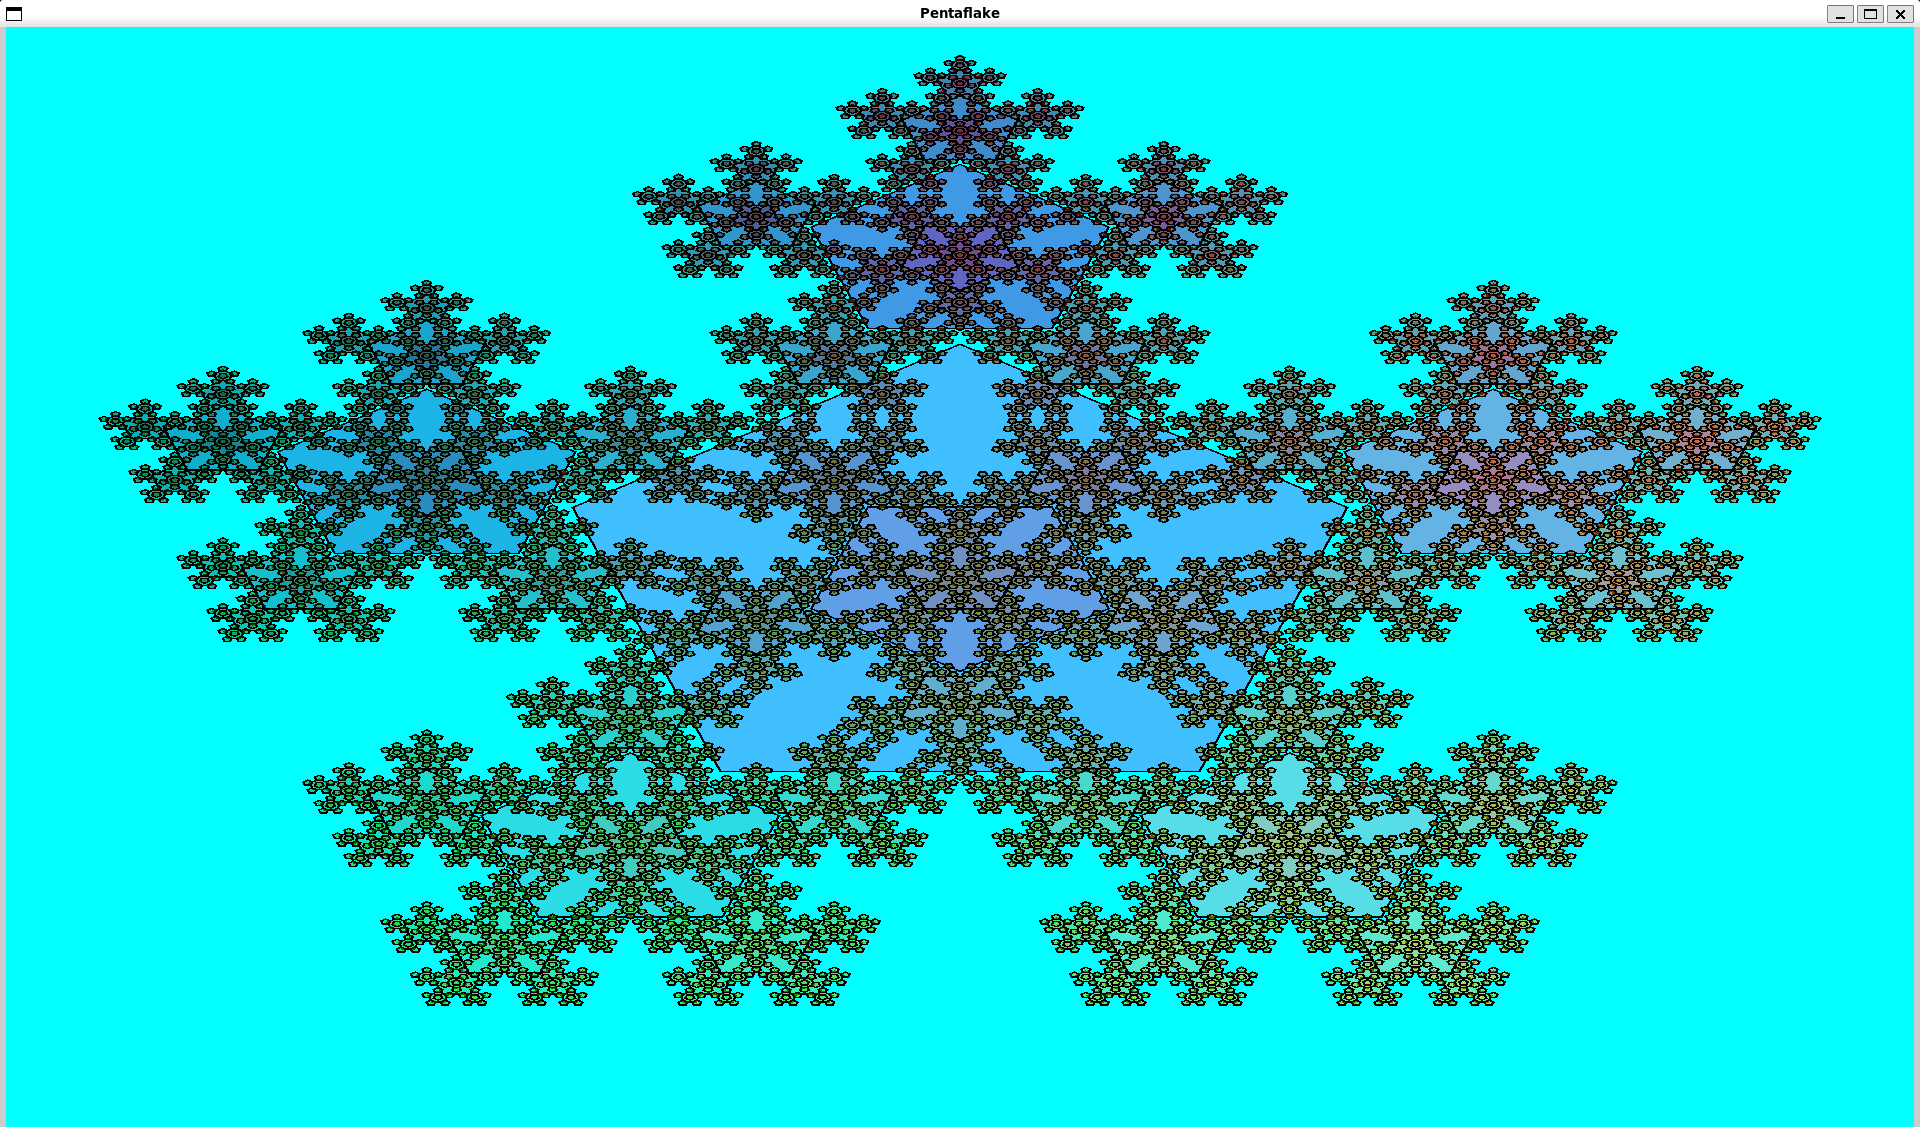
\includegraphics[width=10cm]{comp 4/images/ps2_screenshot.png}
	\caption{My Pentaflake}
	
\end{figure}
\newpage
% PS2: Pentaflake
\section{PS3 :Static N-body Simulation \& Dynamic N-body Simulation}
\subsection{Overview}
I developed an N-Body Simulation program using SFML that models the motion of celestial bodies in a universe. The project simulates gravitational interactions between particles, allowing users to visualize planetary movements based on Newton's laws of motion and gravitation
\subsection{What I Accomplished}
1.I have used SFML for graphical rendering, allowing dynamic visualization of planetary movements.
\newline
2. I have Developed a Universe class to manage multiple celestial bodies and their interactions.
\newline
3. I have Implemented a CelestialBody class to represent individual celestial objects with position, velocity, and mass properties.
\subsection{What I Learned}
==$>$I have learned how to implement graphics and animations using sfml.
\newline
==$>$I have learned some concepts of physics
\subsection{Discussion of Key Algorithms}
\textbf{Data Structures:}
\newline
1.sf::Vector2f:
\newline
for position and velocity representation
\newline
2.sf::Sprite and sf::Texture 
\newline
for graphical rendering
\newline
\textbf{Algorithms:}
\newline
1. Gravitational Force Calculation:
\newline
The gravitational force between two celestial bodies is calculated using Newton's law of universal gravitation:

\[
F = \frac{G \cdot m_1 \cdot m_2}{r^2}
\]

Where:
\begin{itemize}
    \item \( F \) is the gravitational force between the two bodies,
    \item \( G \) is the gravitational constant (\(6.67430 \times 10^{-11} \, \text{m}^3 \, \text{kg}^{-1} \, \text{s}^{-2}\)),
    \item \( m_1 \) and \( m_2 \) are the masses of the two bodies,
    \item \( r \) is the distance between the centers of the two bodies.
\end{itemize}


2. Position and Velocity Update:
\newline
 ==$>$By Applying Newton's laws of motion i have calculated the position and velocity.
\newline
\textbf{Object Oriented Designs:}
\newline
==$>$Inheritance:
\newline
The Universe class is inherited from sf::Drawable (SFML class), which is used to draw it  onto an SFML window.
\newline
==$>$Friend Functions:
\newline
The operator>> and operator<< for Universe are implemented as friend functions.
\subsection{What I Already Knew}
==$>$I was familiar with basic physics concepts.
\newline
==$>$I have learned Use of sfml from previous projects.
\subsection{Challenges}
==$>$I have faced difficulty in implementing the correct gravitational force between each planets.
\newline
==$>$I have faced difficulty in Drawing and updating all the celestial bodies.
\newline
==$>$I have faced difficulty in setting the initial velocity and positions.

\subsection{Codes}

\subsubsection{Makefile}
\begin{lstlisting}[style=cppcode]
CXX = g++
CXXFLAGS = -std=c++17 -Wall -Wextra -pedantic -Werror
SFML_LIBS = -lsfml-graphics -lsfml-window -lsfml-system -lsfml-audio

all: NBody NBody.a test

NBody: main.o Universe.o CelestialBody.o
	$(CXX) $(CXXFLAGS) -o $@ $^ $(SFML_LIBS)

NBody.a: Universe.o CelestialBody.o
	ar rcs $@ $^

main.o: main.cpp Universe.hpp CelestialBody.hpp
	$(CXX) $(CXXFLAGS) -c $<

Universe.o: Universe.cpp Universe.hpp CelestialBody.hpp
	$(CXX) $(CXXFLAGS) -c $<

CelestialBody.o: CelestialBody.cpp CelestialBody.hpp
	$(CXX) $(CXXFLAGS) -c $<

test: test.cpp Universe.o CelestialBody.o
	$(CXX) $(CXXFLAGS) -o $@ $^ $(SFML_LIBS)

lint:
	cpplint --filter=-legal/copyright *.cpp *.hpp

clean:
	rm -f *.o NBody NBody.a test

.PHONY: all clean lint test
\end{lstlisting}
\subsubsection{main.cpp}
\begin{lstlisting}[style=cppcode]
// CopyRight [2024] Ashish Kosana
#include <iostream>
#include <iomanip>
#include <sstream>
#include "Universe.hpp"
#include <SFML/Graphics.hpp>
#include <SFML/Audio.hpp>

// Function to draw a digit using rectangles
void drawDigit(sf::RenderWindow& window, int digit, float x, float y, float size) {
    const bool segments[10][7] = {
        {1, 1, 1, 0, 1, 1, 1},  // 0
        {0, 0, 1, 0, 0, 1, 0},  // 1
        {1, 0, 1, 1, 1, 0, 1},  // 2
        {1, 0, 1, 1, 0, 1, 1},  // 3
        {0, 1, 1, 1, 0, 1, 0},  // 4
        {1, 1, 0, 1, 0, 1, 1},  // 5
        {1, 1, 0, 1, 1, 1, 1},  // 6
        {1, 0, 1, 0, 0, 1, 0},  // 7
        {1, 1, 1, 1, 1, 1, 1},  // 8
        {1, 1, 1, 1, 0, 1, 1}   // 9
    };

    sf::RectangleShape rect;
    rect.setFillColor(sf::Color::White);

    // Draw the segments
    if (segments[digit][0]) {
        rect.setSize(sf::Vector2f(size, size/5));
        rect.setPosition(x, y);
        window.draw(rect);
    }
    if (segments[digit][1]) {
        rect.setSize(sf::Vector2f(size/5, size));
        rect.setPosition(x, y);
        window.draw(rect);
    }
    if (segments[digit][2]) {
        rect.setSize(sf::Vector2f(size/5, size));
        rect.setPosition(x+size-size/5, y);
        window.draw(rect);
    }
    if (segments[digit][3]) {
        rect.setSize(sf::Vector2f(size, size/5));
        rect.setPosition(x, y+size-size/5);
        window.draw(rect);
    }
    if (segments[digit][4]) {
        rect.setSize(sf::Vector2f(size/5, size));
        rect.setPosition(x, y+size);
        window.draw(rect);
    }
    if (segments[digit][5]) {
        rect.setSize(sf::Vector2f(size/5, size));
        rect.setPosition(x+size-size/5, y+size);
        window.draw(rect);
    }
    if (segments[digit][6]) {
        rect.setSize(sf::Vector2f(size, size/5));
        rect.setPosition(x, y+size*2-size/5);
        window.draw(rect);
    }
}

// Function to draw "sec" using rectangles
void drawSec(sf::RenderWindow& window, float x, float y, float size) {
    sf::RectangleShape rect;
    rect.setFillColor(sf::Color::White);

    // Draw 's'
    rect.setSize(sf::Vector2f(size, size/5));
    rect.setPosition(x, y);
    window.draw(rect);
    rect.setPosition(x, y + size/2);
    window.draw(rect);
    rect.setPosition(x, y + size - size/5);
    window.draw(rect);
    rect.setSize(sf::Vector2f(size/5, size/2));
    rect.setPosition(x, y);
    window.draw(rect);
    rect.setPosition(x + size - size/5, y + size/2);
    window.draw(rect);

    // Draw 'e'
    x += size * 1.2;
    rect.setSize(sf::Vector2f(size, size/5));
    rect.setPosition(x, y);
    window.draw(rect);
    rect.setPosition(x, y + size/2);
    window.draw(rect);
    rect.setPosition(x, y + size - size/5);
    window.draw(rect);
    rect.setSize(sf::Vector2f(size/5, size/2 + size/5));
    rect.setPosition(x, y);
    window.draw(rect);
    rect.setSize(sf::Vector2f(size, size/5));
    rect.setPosition(x, y + size/2);
    window.draw(rect);

    // Draw 'c'
    x += size * 1.2;
    rect.setSize(sf::Vector2f(size, size/5));
    rect.setPosition(x, y);
    window.draw(rect);
    rect.setPosition(x, y + size - size/5);
    window.draw(rect);
    rect.setSize(sf::Vector2f(size/5, size));
    rect.setPosition(x, y);
    window.draw(rect);
}

int main(int argc, char* argv[]) {
    if (argc != 3) {
        std::cerr << "Usage: " << argv[0] << " <T> <dt>" << std::endl;
        return 1;
    }

    double T = std::stod(argv[1]);
    double dt = std::stod(argv[2]);

    NB::Universe universe;
    std::cin >> universe;

    // Create render window
    sf::RenderWindow window(sf::VideoMode(800, 800), "ASHISH'S SOLAR SYSTEM");

    // Set vertical sync enabled (no return value check, since it's void)
    window.setVerticalSyncEnabled(true);

    double viewSize = universe.getRadius() * 2.5e-9;
    sf::View universeView(sf::Vector2f(0, 0), sf::Vector2f(static_cast<float>(viewSize),
                          static_cast<float>(viewSize)));
    sf::View defaultView = window.getDefaultView();

    // Load background texture
    sf::Texture backgroundTexture;
    if (!backgroundTexture.loadFromFile("starfield.jpg")) {
        std::cerr << "Failed to load background image" << std::endl;
        return 1;
    }
    sf::Sprite background(backgroundTexture);

    // Load and play music
    sf::Music music;
    if (!music.openFromFile("2001.wav")) {
        std::cerr << "Failed to load music file" << std::endl;
        return 1;
    }
    music.setLoop(true);
    music.play();
    std::cout << "Music started playing." << std::endl;

    // Scale and position the background
    background.setScale(
        static_cast<float>(viewSize) / backgroundTexture.getSize().x,
        static_cast<float>(viewSize) / backgroundTexture.getSize().y);
    background.setPosition(static_cast<float>(-viewSize/2), static_cast<float>(-viewSize/2));

    // Setup for displaying elapsed time using shapes
    sf::RectangleShape timeBox(sf::Vector2f(150, 50));
    timeBox.setFillColor(sf::Color(0, 0, 0, 128));
    timeBox.setPosition(defaultView.getSize().x - 160, 10);

    sf::Clock clock;
    double elapsedTime = 0.0;
    bool firstDraw = true;

    // Main window loop
    while (window.isOpen() && elapsedTime < T) {
        sf::Event event;
        while (window.pollEvent(event)) {
            if (event.type == sf::Event::Closed) {
                window.close();
            }
            if (event.type == sf::Event::KeyPressed && event.key.code == sf::Keyboard::S) {
                if (music.getStatus() == sf::Music::Playing) {
                    music.pause();
                    std::cout << "Music paused" << std::endl;
                } else {
                    music.play();
                    std::cout << "Music resumed" << std::endl;
                }
            }
        }

        // Calculate frame time
        double frameTime = clock.restart().asSeconds();
        elapsedTime += frameTime;

        // Update universe state
        universe.step(dt);

        // Clear and draw everything
        window.clear();

        // Draw universe
        window.setView(universeView);
        window.draw(background);
        window.draw(universe);

        // Draw time
        window.setView(defaultView);
        window.draw(timeBox);

        // Display elapsed time in simulation
        int seconds = static_cast<int>(elapsedTime);
        int tens = seconds / 10;
        int ones = seconds % 10;

        drawDigit(window, tens, defaultView.getSize().x - 150, 15, 20);
        drawDigit(window, ones, defaultView.getSize().x - 120, 15, 20);

        // Draw "sec" for seconds
        drawSec(window, defaultView.getSize().x - 90, 15, 20);

        if (firstDraw) {
            std::cout << "Drawing universe for the first time" << std::endl;
            firstDraw = false;
        }

        // Display rendered frame
        window.display();
    }

    // Output universe state at the end
    std::cout << universe;

    return 0;
}
\end{lstlisting}
\subsubsection{CelestialBody.hpp}
\begin{lstlisting}[style=cppcode]
// CopyRight [2024] Ashish Kosana
#pragma once
#include <memory>
#include <string>
#include <SFML/Graphics.hpp>

namespace NB {

class CelestialBody : public sf::Drawable {
 public:
    CelestialBody();
    CelestialBody(double x, double y, double vx, double vy, double mass,
                  const std::string& filename);

    void update(double dt);
    sf::Vector2f getPosition() const;
    sf::Vector2f getVelocity() const;
    double getMass() const;

    void setVelocity(const sf::Vector2f& newVelocity);
    void setPosition(const sf::Vector2f& newPosition);
    void applyForce(const sf::Vector2f& force, double dt);

    friend std::istream& operator>>(std::istream& is, CelestialBody& body);
    friend std::ostream& operator<<(std::ostream& os, const CelestialBody& body);

 protected:
    void draw(sf::RenderTarget& target, sf::RenderStates states) const override;

 private:
    sf::Vector2f position;
    sf::Vector2f velocity;
    double mass;
    sf::Texture texture;
    mutable sf::Sprite sprite;
    static constexpr float SCALE = 1e-9f;
    static constexpr double G = 6.67430e-11;
};

}  // namespace NB

\end{lstlisting}
\subsubsection{CelestialBody.cpp}
\begin{lstlisting}[style=cppcode]
// CopyRight [2024] Ashish Kosana
#include "CelestialBody.hpp"
#include <iostream>

namespace NB {

CelestialBody::CelestialBody() : mass(0) {}

CelestialBody::CelestialBody(double x, double y, double vx, double vy, double m,
const std::string& filename)
: position(x, y), velocity(vx, vy), mass(m) {
if (!texture.loadFromFile(filename)) {
std::cerr << "Failed to load texture: " << filename << std::endl;
}
sprite.setTexture(texture);
sprite.setOrigin(sprite.getLocalBounds().width / 2, sprite.getLocalBounds().height / 2);
sprite.setPosition(position.x * SCALE, position.y * SCALE);
}

void CelestialBody::update(double dt) {
position += velocity * static_cast<float>(dt);
sprite.setPosition(position.x * SCALE, position.y * SCALE);
}

sf::Vector2f CelestialBody::getPosition() const {
return position;
}

sf::Vector2f CelestialBody::getVelocity() const {
return velocity;
}

double CelestialBody::getMass() const {
return mass;
}

void CelestialBody::setVelocity(const sf::Vector2f& newVelocity) {
velocity = newVelocity;
}

void CelestialBody::setPosition(const sf::Vector2f& newPosition) {
position = newPosition;
sprite.setPosition(position.x * SCALE, position.y * SCALE);
}

void CelestialBody::applyForce(const sf::Vector2f& force, double dt) {
sf::Vector2f acceleration = force / static_cast<float>(mass);
velocity += acceleration * static_cast<float>(dt);
}

void CelestialBody::draw(sf::RenderTarget& target, sf::RenderStates states) const {
target.draw(sprite, states);
}

std::istream& operator>>(std::istream& is, CelestialBody& body) {
std::string filename;
is >> body.position.x >> body.position.y >> body.velocity.x >> body.velocity.y
>> body.mass >> filename;
if (!body.texture.loadFromFile(filename)) {
std::cerr << "Failed to load texture: " << filename << std::endl;
}
body.sprite.setTexture(body.texture);
body.sprite.setOrigin(body.sprite.getLocalBounds().width / 2,
body.sprite.getLocalBounds().height / 2);
body.sprite.setPosition(body.position.x * body.SCALE, body.position.y * body.SCALE);
return is;
}

std::ostream& operator<<(std::ostream& os, const CelestialBody& body) {
os << body.position.x << " " << body.position.y << " "
<< body.velocity.x << " " << body.velocity.y << " "
<< body.mass << " " << "image.png";  // Assuming image filename
return os;
}

}  // namespace NB

\end{lstlisting}
\subsubsection{Universe.hpp}
\begin{lstlisting}[style=cppcode]
// CopyRight [2024] Ashish Kosana
#pragma once

#include <vector>
#include <memory>
#include "CelestialBody.hpp"
#include <SFML/Graphics/Drawable.hpp>

namespace NB {

class Universe : public sf::Drawable {
 public:
    Universe();
    explicit Universe(const std::string& filename);

    void update(double dt);
    void step(double seconds);
    size_t size() const;
    double getRadius() const;
    const CelestialBody& operator[](size_t index) const;

    friend std::istream& operator>>(std::istream& is, Universe& universe);
    friend std::ostream& operator<<(std::ostream& os, const Universe& universe);

 protected:
    void draw(sf::RenderTarget& target, sf::RenderStates states) const override;

 private:
    std::vector<std::unique_ptr<CelestialBody>> bodies;
    double radius;
    sf::Vector2f calculateForce(const CelestialBody& body1, const CelestialBody& body2) const;
};

}  // namespace NB


\end{lstlisting}
\subsubsection{Universe.cpp}
\begin{lstlisting}[style=cppcode]
// CopyRight [2024] Ashish Kosana
#include "Universe.hpp"
#include <fstream>
#include <iostream>
#include <cmath>

namespace NB {

Universe::Universe() : radius(0) {}

Universe::Universe(const std::string& filename) {
std::ifstream file(filename);
if (file) {
file >> *this;
} else {
std::cerr << "Failed to open file: " << filename << std::endl;
}
}

void Universe::update(double dt) {
for (auto& body : bodies) {
body->update(dt);
}
}

void Universe::step(double seconds) {
for (auto& body : bodies) {
sf::Vector2f totalForce(0, 0);
for (const auto& otherBody : bodies) {
if (body.get() != otherBody.get()) {
totalForce += calculateForce(*body, *otherBody);
}
}
body->applyForce(totalForce, seconds);
}

for (auto& body : bodies) {
body->update(seconds);
}
}

size_t Universe::size() const { return bodies.size(); }
double Universe::getRadius() const { return radius; }

const CelestialBody& Universe::operator[](size_t index) const {
return *bodies[index];
}

void Universe::draw(sf::RenderTarget& target, sf::RenderStates states) const {
for (const auto& body : bodies) {
target.draw(*body, states);
}
}

sf::Vector2f Universe::calculateForce(const CelestialBody& body1,
const CelestialBody& body2) const {
sf::Vector2f delta = body2.getPosition() - body1.getPosition();
double distance = std::sqrt(delta.x * delta.x + delta.y * delta.y);
double force = (6.67430e-11 * body1.getMass() * body2.getMass()) / (distance * distance);
return (delta / static_cast<float>(distance)) * static_cast<float>(force);
}

std::istream& operator>>(std::istream& is, Universe& universe) {
size_t n;
is >> n >> universe.radius;
universe.bodies.clear();
for (size_t i = 0; i < n; ++i) {
auto body = std::make_unique<CelestialBody>();
is >> *body;
universe.bodies.push_back(std::move(body));
}
return is;
}

std::ostream& operator<<(std::ostream& os, const Universe& universe) {
os << universe.bodies.size() << " " << universe.radius << "\n";
for (const auto& body : universe.bodies) {
os << *body << "\n";
}
return os;
}

}  // namespace NB

\end{lstlisting}

\subsubsection{test.cpp}
\begin{lstlisting}[style=cppcode]
// CopyRight [2024] Ashish Kosana
#define BOOST_TEST_MODULE NBodyTests
#include <sstream>
#include <boost/test/included/unit_test.hpp>
#include "Universe.hpp"
#include "CelestialBody.hpp"

const float EPSILON = 1e-6f;

BOOST_AUTO_TEST_CASE(CelestialBodyInputOutput) {
    std::stringstream ss("1.496e+11 0 0 29800 5.974e+24 earth.gif");
    NB::CelestialBody body;
    ss >> body;

    BOOST_CHECK_CLOSE(body.getPosition().x, 1.496e+11f, EPSILON);
    BOOST_CHECK_SMALL(body.getPosition().y, EPSILON);
    BOOST_CHECK_SMALL(body.getVelocity().x, EPSILON);
    BOOST_CHECK_CLOSE(body.getVelocity().y, 29800.0f, EPSILON);
    BOOST_CHECK_CLOSE(body.getMass(), 5.974e+24f, EPSILON);

    std::stringstream out;
    out << body;
    BOOST_CHECK_EQUAL(out.str(), "1.496e+11 0 0 29800 5.974e+24 image.png");
}

BOOST_AUTO_TEST_CASE(UniverseInitialization) {
    NB::Universe universe;
    BOOST_CHECK_EQUAL(universe.size(), 0);
    BOOST_CHECK_SMALL(static_cast<float>(universe.getRadius()), EPSILON);
}

BOOST_AUTO_TEST_CASE(UniverseInputOutput) {
    std::stringstream ss("1 2.50e+11\n1.496e+11 0 0 29800 5.974e+24 mars.gif\n");
    NB::Universe universe;
    ss >> universe;

    BOOST_CHECK_EQUAL(universe.size(), 1);
    BOOST_CHECK_CLOSE(static_cast<float>(universe.getRadius()), 2.50e+11f, EPSILON);

    std::stringstream out;
    out << universe;
    BOOST_CHECK_EQUAL(out.str(), "1 2.5e+11\n1.496e+11 0 0 29800 5.974e+24 image.png\n");
}

BOOST_AUTO_TEST_CASE(UniverseAccessOperator) {
    std::stringstream ss("1 2.50e+11\n1.496e+11 0 0 29800 5.974e+24 mercury.gif\n");
    NB::Universe universe;
    ss >> universe;

    BOOST_CHECK_CLOSE(universe[0].getPosition().x, 1.496e+11f, EPSILON);
    BOOST_CHECK_SMALL(universe[0].getPosition().y, EPSILON);
    BOOST_CHECK_SMALL(universe[0].getVelocity().x, EPSILON);
    BOOST_CHECK_CLOSE(universe[0].getVelocity().y, 29800.0f, EPSILON);
    BOOST_CHECK_CLOSE(universe[0].getMass(), 5.974e+24f, EPSILON);
}

BOOST_AUTO_TEST_CASE(UniverseSimulationStep) {
    std::stringstream ss("1 2.50e+11\n1.496e+11 0 0 29800 5.974e+24 sun.gif\n");
    NB::Universe universe;
    ss >> universe;

    BOOST_CHECK_CLOSE(universe[0].getPosition().x, 1.496e+11f, EPSILON);
    BOOST_CHECK_SMALL(universe[0].getPosition().y, EPSILON);

    universe.step(1.0);

    BOOST_CHECK_CLOSE(universe[0].getPosition().x, 1.496e+11f, EPSILON);
    BOOST_CHECK_CLOSE(universe[0].getPosition().y, 29800.0f, EPSILON);
}

BOOST_AUTO_TEST_CASE(UniverseMultipleBodies) {
    std::stringstream ss("3 2.50e+11\n"
                         "1.496e+11 0 0 29800 5.974e+24 saturn.gif\n"
                         "2.279e+11 0 0 24100 6.419e+23 pluto.gif\n"
                         "5.790e+10 0 0 47900 3.302e+23 uranus.gif\n");
    NB::Universe universe;
    ss >> universe;

    BOOST_CHECK_EQUAL(universe.size(), 3);
    BOOST_CHECK_CLOSE(static_cast<float>(universe.getRadius()), 2.50e+11f, EPSILON);

    // Check Earth
    BOOST_CHECK_CLOSE(universe[0].getPosition().x, 1.496e+11f, EPSILON);
    BOOST_CHECK_CLOSE(universe[0].getVelocity().y, 29800.0f, EPSILON);
    BOOST_CHECK_CLOSE(universe[0].getMass(), 5.974e+24f, EPSILON);

    // Check Mars
    BOOST_CHECK_CLOSE(universe[1].getPosition().x, 2.279e+11f, EPSILON);
    BOOST_CHECK_CLOSE(universe[1].getVelocity().y, 24100.0f, EPSILON);
    BOOST_CHECK_CLOSE(universe[1].getMass(), 6.419e+23f, EPSILON);

    // Check Mercury
    BOOST_CHECK_CLOSE(universe[2].getPosition().x, 5.790e+10f, EPSILON);
    BOOST_CHECK_CLOSE(universe[2].getVelocity().y, 47900.0f, EPSILON);
    BOOST_CHECK_CLOSE(universe[2].getMass(), 3.302e+23f, EPSILON);

    universe.step(1.0);

    // Check updated positions
    BOOST_CHECK_CLOSE(universe[0].getPosition().y, 29800.0f, EPSILON);
    BOOST_CHECK_CLOSE(universe[1].getPosition().y, 24100.0f, EPSILON);
    BOOST_CHECK_CLOSE(universe[2].getPosition().y, 47900.0f, EPSILON);
}

// New test case for physics simulation
BOOST_AUTO_TEST_CASE(PhysicsSimulation) {
    std::stringstream ss("2 2.50e+11\n"
                         "0 0 0 0 1.989e+30 sun.gif\n"
                         "1.496e+11 0 0 29800 5.974e+24 earth.gif\n");
    NB::Universe universe;
    ss >> universe;

    BOOST_CHECK_EQUAL(universe.size(), 2);

    // Initial positions
    BOOST_CHECK_SMALL(universe[0].getPosition().x, EPSILON);
    BOOST_CHECK_SMALL(universe[0].getPosition().y, EPSILON);
    BOOST_CHECK_CLOSE(universe[1].getPosition().x, 1.496e+11f, EPSILON);
    BOOST_CHECK_SMALL(universe[1].getPosition().y, EPSILON);

    // Simulate for 1 day
    double dt = 86400;  // 1 day in seconds
    universe.step(dt);

    // Check that the sun has not moved significantly
    BOOST_CHECK_SMALL(universe[0].getPosition().x, 1e5f);
    BOOST_CHECK_SMALL(universe[0].getPosition().y, 1e5f);

    // Check that the Earth has moved
    BOOST_CHECK_CLOSE(universe[1].getPosition().x, 1.496e+11f, 1.0f);
    BOOST_CHECK(std::abs(universe[1].getPosition().y) > 2.5e+9f);

    // Check that the Earth's velocity has changed slightly due to the sun's gravity
    BOOST_CHECK(universe[1].getVelocity().x < 0);
    BOOST_CHECK_CLOSE(universe[1].getVelocity().y, 29800.0f, 1.0f);
}

\end{lstlisting}
\newpage
\subsubsection{Screenshot}
\begin{figure}[tbh]
	\centering
	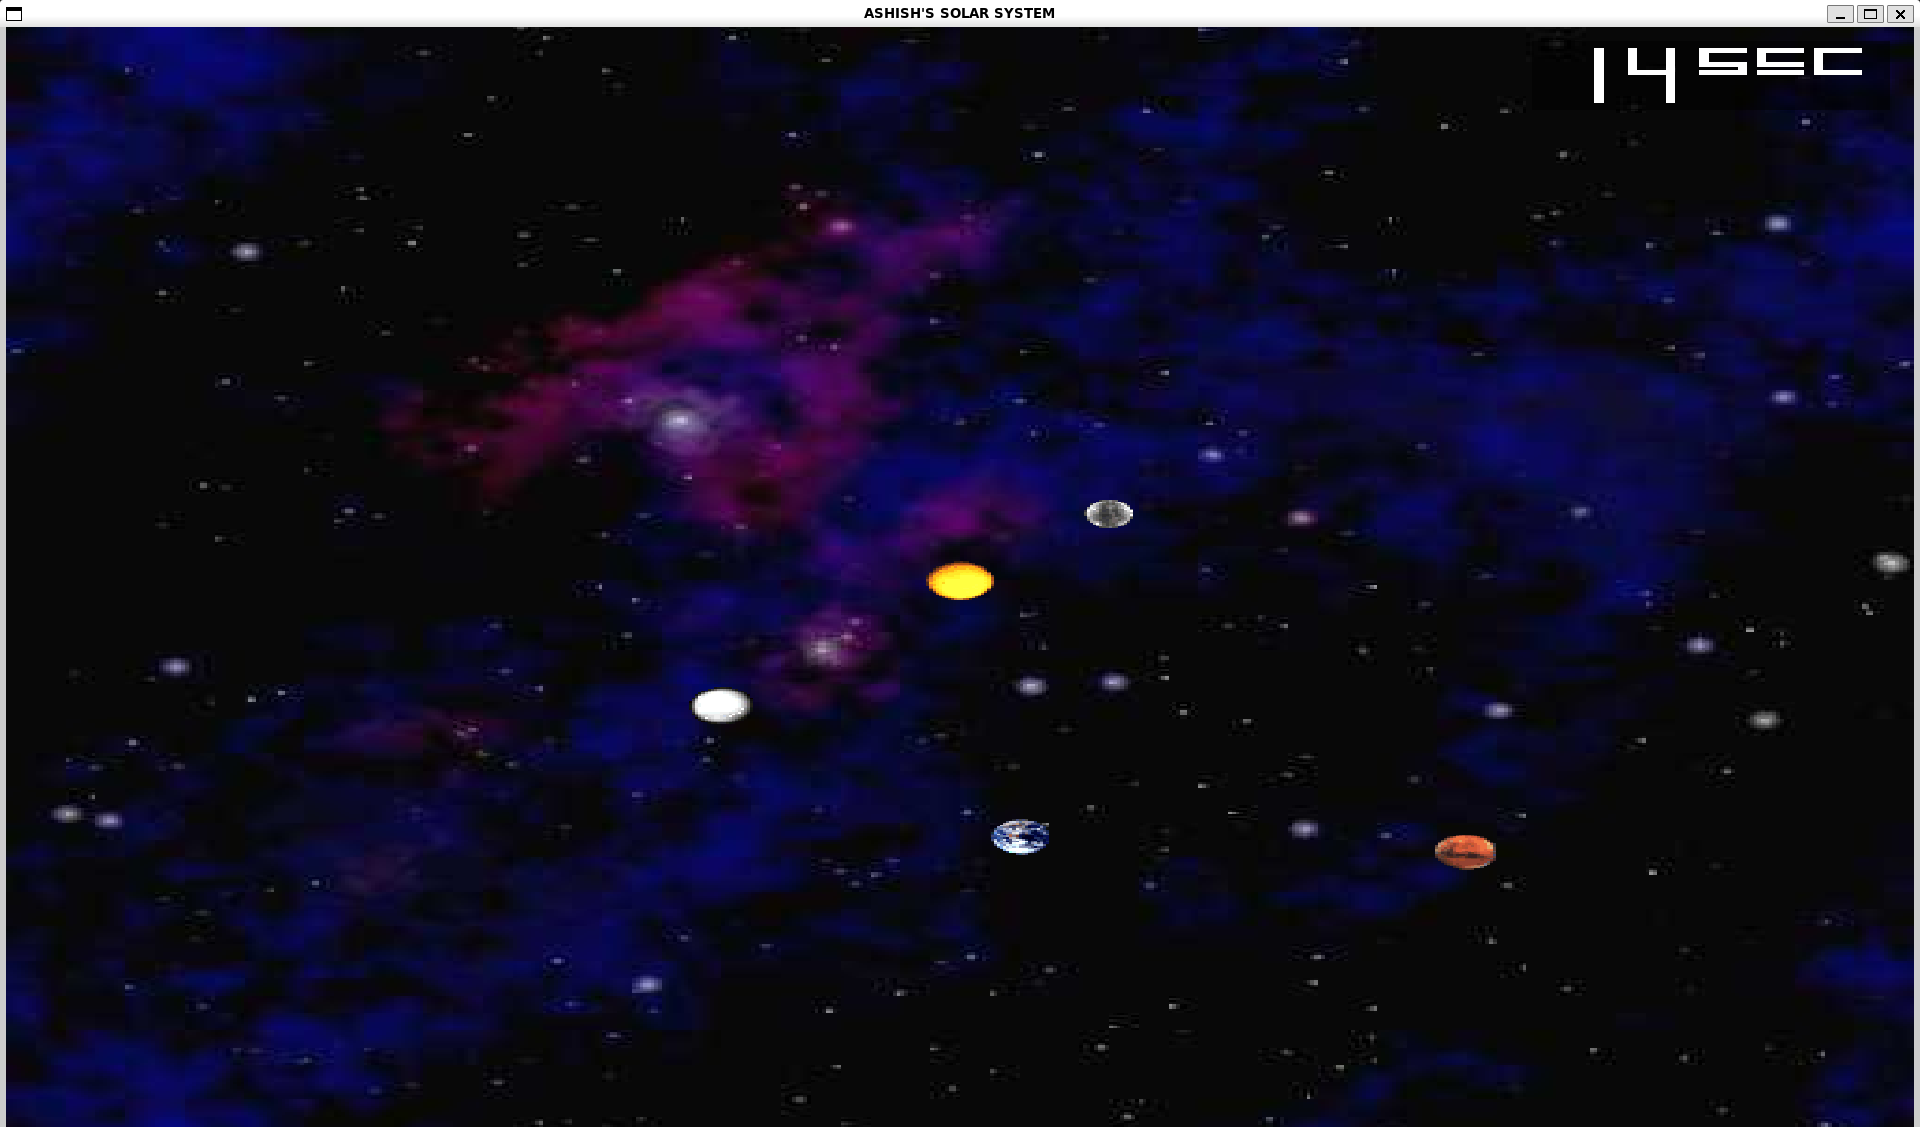
\includegraphics[width=10cm]{comp 4/images/ps3b_screenshot.png}
	\caption{My Solar System}
\end{figure}
% PS3a \& ps3b :Static N-body Simulation \& Dynamic N-body Simulation
\newpage
\section{PS4: Sokoban UI \& Sokoban}
\subsection{Overview}
I implemented a Sokoban game using C++ and SFML, implementing the core mechanics of this classic puzzle game. The project involved creating a game board, handling player movement, and managing box pushing mechanics.
\subsection{What I Accomplished}
1.Implemented level loading from text files, allowing for easy addition of new puzzles
\newline
2.Implemented a win condition check to determine when the player has completed the level
\newline
3.Developed a rendering system using SFML to display the game board, player, boxes, and storage locations
\subsection{What I Learned}
==>I have learned how to handle the user inputs and event processing.
\newline
==$>$Rendering game elements using sprites
\subsection{Discussion of Key Algorithms}
\textbf{Data Structures:}
\newline
1.sf::Vector2i 
\newline
==$>$Represents the player's current position on the game board.
\newline
2.sf::Sprite Array:
\newline
Includes sprites for ground, walls, boxes, storage locations, and player.
\newline
3. sf::Texture Array:
\newline
==$>$Stores textures for game elements.
\newline
==$>$Corresponds to the sprite array for efficient texture management.
\newline
\textbf{Algorithms:}
\newline
1.Player Movement Algorithm:
\newline
==$>$Checks for valid moves based on surrounding cells.
\newline
==$>$Updates player position and box positions if applicable.
\newline
2. Win Condition Checking:
\newline
==$>$Iterates through the game board to verify if all boxes are on storage locations.
\newline
\textbf{Object Oriented Designs:}
\newline
==$>$Class:
\newline
The sokoban class represents the core game logic and contains the member variables.
\newline
==$>$Operator Overloading:
\newline
The operator<< and operator>> for Sokoban and sf::Vector2 are overloaded to handle input and output operations properly.
\subsection{What I Already Knew}
==$>$I have idead about c++ file handling.
\newline
==$>$I have grip over sfml ,that how to load the textures etc from previous projects.
\subsection{Challenges}
==$>$I have faced difficulty in implementing the logic for pushing the boxes on to the storage areas and preventing the player not to push the boxes on to the blocked area.
\newline
==$>$I have faced some difficulty in implementing the undo logic.
\newline
==$>$I have also faced difficulty in implementing the victory where the user gets congratulations you won the game on the window.
\newline
==$>$I have faced little difficulty in playing the victory music by checking the win condition.

\subsection{Codes}

\subsubsection{Makefile}
\begin{lstlisting}[style=cppcode]
CXX = g++
CXXFLAGS = -std=c++20 -Wall -Werror -pedantic -g
SFML_LIBS = -lsfml-graphics -lsfml-audio -lsfml-window -lsfml-system
BOOST_LIBS = -lboost_unit_test_framework

SRCS = Sokoban.cpp main.cpp
OBJS = $(SRCS:.cpp=.o)

HDRS = Sokoban.hpp

all: Sokoban Sokoban.a test

Sokoban: $(OBJS)
	$(CXX) $(CXXFLAGS) -o $@ $^ $(SFML_LIBS)

Sokoban.a: Sokoban.o
	ar rcs $@ $^

test: test.o Sokoban.o
	$(CXX) $(CXXFLAGS) -o $@ $^ $(SFML_LIBS) $(BOOST_LIBS)

%.o: %.cpp $(HDRS)
	$(CXX) $(CXXFLAGS) -c $< -o $@

lint:
	cpplint --filter=-legal/copyright *.cpp *.hpp

clean:
	rm -f *.o Sokoban Sokoban.a test

.PHONY: all lint clean test
\end{lstlisting}
\subsubsection{main.cpp}
\begin{lstlisting}[style=cppcode]
// Copyright [2024] Ashish Kosana
#include <iostream>
#include <fstream>
#include <sstream>
#include <iomanip>
#include <SFML/Graphics.hpp>
#include <SFML/Audio.hpp>  // Include SFML Audio module
#include "Sokoban.hpp"

// Function to load best time from file
int loadBestTime(const std::string& levelName) {
    std::ifstream file(levelName + "_best_time.txt");
    int bestTime = -1;
    if (file >> bestTime) {
        return bestTime;
    }
    return -1;  // If no time is recorded, return -1
}

// Function to save best time to file
void saveBestTime(const std::string& levelName, int bestTime) {
    std::ofstream file(levelName + "_best_time.txt");
    file << bestTime;
}

int main(int argc, char* argv[]) {
    if (argc != 2) {
        std::cerr << "Usage: " << argv[0] << " <level_file>" << std::endl;
        return 1;
    }

    SB::Sokoban game(argv[1]);
    sf::RenderWindow window(sf::VideoMode(game.pixelWidth(),
    game.pixelHeight()), "ASHISH'S SOKOBAN");

    // Load font
    sf::Font font;
    if (!font.loadFromFile("arialn.ttf")) {
        std::cerr << "Error loading font" << std::endl;
        return 1;
    }

    // Load victory music
    sf::Music victoryMusic;
    if (!victoryMusic.openFromFile("victory.wav")) {
        std::cerr << "Error loading victory music" << std::endl;
        return 1;
    }

    // Timer and reset texts
    sf::Text timerText("", font, 20);
    timerText.setFillColor(sf::Color::White);
    timerText.setPosition(10, 10);

    // Move counter text
    sf::Text moveCounterText("Moves: 0", font, 20);
    moveCounterText.setFillColor(sf::Color::White);
    moveCounterText.setPosition(10, 40);

    // Best time display
    sf::Text bestTimeText("Best Time: --:--", font, 20);
    bestTimeText.setFillColor(sf::Color::Yellow);
    bestTimeText.setPosition(10, 70);

    // Load the best time from file
    int bestTime = loadBestTime(argv[1]);
    if (bestTime != -1) {
        int bestMinutes = bestTime / 60;
        int bestSeconds = bestTime % 60;
        std::stringstream bestTimeStream;
        bestTimeStream << "Best Time: " << std::setw(2) << std::setfill('0')
                       << bestMinutes << ":" << std::setw(2) << std::setfill('0')
                       << bestSeconds;
        bestTimeText.setString(bestTimeStream.str());
    }

    sf::Clock clock;
    int moveCount = 0;
    bool gameWon = false;
    bool musicPlayed = false;  // Flag to check if music has been played

    while (window.isOpen()) {
        sf::Event event;
        while (window.pollEvent(event)) {
            if (event.type == sf::Event::Closed) {
                window.close();
            }
            if (event.type == sf::Event::KeyPressed) {
                if (!gameWon) {
                    switch (event.key.code) {
                        case sf::Keyboard::Up:
                        case sf::Keyboard::W:
                            game.movePlayer(SB::Direction::Up);
                            moveCount++;
                            break;
                        case sf::Keyboard::Down:
                        case sf::Keyboard::S:
                            game.movePlayer(SB::Direction::Down);
                            moveCount++;
                            break;
                        case sf::Keyboard::Left:
                        case sf::Keyboard::A:
                            game.movePlayer(SB::Direction::Left);
                            moveCount++;
                            break;
                        case sf::Keyboard::Right:
                        case sf::Keyboard::D:
                            game.movePlayer(SB::Direction::Right);
                            moveCount++;
                            break;
                        case sf::Keyboard::U:  // Undo move
                            game.undo();
                            if (moveCount > 0) moveCount--;
                            break;
                        case sf::Keyboard::R:  // Reset game
                            game.reset();
                            clock.restart();
                            moveCount = 0;
                            musicPlayed = false;  // Reset music played flag
                            victoryMusic.stop();  // Stop music if playing
                            break;
                        default:
                            break;
                    }
                }
                // Check for reset after winning
                if (gameWon && event.key.code == sf::Keyboard::R) {
                    game.reset();
                    clock.restart();
                    moveCount = 0;
                    gameWon = false;  // Reset gameWon status to allow playing again
                    musicPlayed = false;  // Reset music played flag
                    victoryMusic.stop();  // Stop music if playing
                }
            }
        }

        window.clear();
        window.draw(game);

        // Update timer display
        int seconds = static_cast<int>(clock.getElapsedTime().asSeconds());
        int minutes = seconds / 60;
        seconds %= 60;
        std::stringstream timeStream;
        timeStream << std::setw(2) << std::setfill('0') << minutes
                   << ":" << std::setw(2) << std::setfill('0') << seconds;
        timerText.setString(timeStream.str());
        window.draw(timerText);

        // Update move counter display
        std::stringstream moveStream;
        moveStream << "Moves: " << moveCount;
        moveCounterText.setString(moveStream.str());
        window.draw(moveCounterText);

        // Display best time
        window.draw(bestTimeText);

        // Check if the game is won and display the win message if true
        if (game.isWon()) {
            gameWon = true;
            sf::Text winText("Congratulations! You won!", font, 30);
            winText.setFillColor(sf::Color::Green);
            winText.setPosition(game.pixelWidth() / 2 - winText.getLocalBounds().width / 2,
                                game.pixelHeight() / 2 - winText.getLocalBounds().height / 2);
            window.draw(winText);

            // Play victory music if not already played
            if (!musicPlayed) {
                victoryMusic.play();
                musicPlayed = true;  // Set flag to indicate music has been played
            }

            // Calculate elapsed time and update best time if necessary
            int elapsedTime = static_cast<int>(clock.getElapsedTime().asSeconds());
            if (bestTime == -1 || elapsedTime < bestTime) {
                bestTime = elapsedTime;
                saveBestTime(argv[1], bestTime);
                bestTimeText.setString("Best Time: "
                + timeStream.str());  // Update best time display
            }
        }

        window.display();
    }

    return 0;
}
\end{lstlisting}
\subsubsection{Sokoban.hpp}
\begin{lstlisting}[style=cppcode]

// Copyright [2024] Ashish Kosana
#ifndef SOKOBAN_HPP
#define SOKOBAN_HPP

#include <ostream>
#include <vector>
#include <string>
#include <stack>
#include <SFML/Graphics.hpp>
#include <SFML/Audio.hpp>
#include <SFML/System/Vector2.hpp>

template <typename T>
std::ostream& operator<<(std::ostream& os, const sf::Vector2<T>& vec);

namespace SB {

enum class Direction { Up, Down, Left, Right };

struct Move {
    sf::Vector2i playerOldPos;
    sf::Vector2i playerNewPos;
    sf::Vector2i boxOldPos;
    sf::Vector2i boxNewPos;
    bool isBoxMove;
};

class Sokoban : public sf::Drawable {
 public:
    Sokoban();
    explicit Sokoban(const std::string& filename);
    int width() const;
    int height() const;
    sf::Vector2i playerLoc() const;
    void movePlayer(Direction dir);
    bool isWon() const;
    void reset();
    int pixelWidth() const;
    int pixelHeight() const;
    void undo();

    friend std::istream& operator>>(std::istream& is, Sokoban& sokoban);
    friend std::ostream& operator<<(std::ostream& os, const Sokoban& sokoban);

 protected:
    void draw(sf::RenderTarget& target, sf::RenderStates states) const override;

 private:
    static const int TILE_SIZE = 64;
    int m_width;
    int m_height;
    std::vector<char> m_grid;
    std::vector<char> m_initialGrid;
    sf::Vector2i m_playerPos;
    sf::Vector2i m_initialPlayerPos;
    sf::Texture m_textures[8];  // Increased for multiple box colors and player directions
    sf::Sprite m_sprites[8];
    Direction m_lastDirection;
    std::stack<Move> m_moveHistory;
    sf::SoundBuffer m_victorySoundBuffer;
    sf::Sound m_victorySound;

    void loadTextures();
    void loadFromFile(const std::string& filename);
    void updatePlayerSprite();
};

}  // namespace SB

#endif  // SOKOBAN_HPP

\end{lstlisting}
\subsubsection{Sokoban.cpp}
\begin{lstlisting}[style=cppcode]
// Copyright [2024] Ashish Kosana
#include "Sokoban.hpp"
#include <iostream>
#include <fstream>
#include <algorithm>

template <typename T>
std::ostream& operator<<(std::ostream& os, const sf::Vector2<T>& vec) {
    os << "(" << vec.x << ", " << vec.y << ")";
    return os;
}

// Explicit instantiation for int
template std::ostream& operator<<(std::ostream&, const sf::Vector2<int>&);

namespace SB {

Sokoban::Sokoban() : m_width(0), m_height(0), m_lastDirection(Direction::Down) {
    loadTextures();
}

Sokoban::Sokoban(const std::string& filename) : m_width(0), m_height(0),
m_lastDirection(Direction::Down) {
    loadTextures();
    loadFromFile(filename);
}

void Sokoban::loadTextures() {
    const std::string textureFiles[] = {
        "ground_01.png", "block_06.png", "crate_03.png", "ground_04.png",
        "player_05.png", "player_20.png", "player_17.png", "player_08.png"
    };

    for (int i = 0; i < 8; ++i) {
        if (!m_textures[i].loadFromFile(textureFiles[i])) {
            std::cerr << "Failed to load " << textureFiles[i] << std::endl;
        }
        m_sprites[i].setTexture(m_textures[i]);
    }
}

int Sokoban::width() const { return m_width; }
int Sokoban::height() const { return m_height; }
sf::Vector2i Sokoban::playerLoc() const { return m_playerPos; }

void Sokoban::movePlayer(Direction dir) {
    sf::Vector2i newPos = m_playerPos;
    switch (dir) {
        case Direction::Up: newPos.y--; break;
        case Direction::Down: newPos.y++; break;
        case Direction::Left: newPos.x--; break;
        case Direction::Right: newPos.x++; break;
    }

    m_lastDirection = dir;
    updatePlayerSprite();

    if (newPos.x >= 0 && newPos.x < m_width &&
        newPos.y >= 0 && newPos.y < m_height) {
        char &targetCell = m_grid[newPos.y * m_width + newPos.x];
        Move move{m_playerPos, newPos, {-1, -1}, {-1, -1}, false};

        if (targetCell == '.' || targetCell == 'a' || targetCell == 'b') {
            std::swap(m_grid[m_playerPos.y * m_width + m_playerPos.x], targetCell);
            m_playerPos = newPos;
            m_moveHistory.push(move);
        } else if (targetCell == 'A' || targetCell == 'B' ||
                   targetCell == '1' || targetCell == '2') {
            sf::Vector2i boxNewPos = newPos + (newPos - m_playerPos);
            if (boxNewPos.x >= 0 && boxNewPos.x < m_width &&
                boxNewPos.y >= 0 && boxNewPos.y < m_height) {
                char &boxTargetCell = m_grid[boxNewPos.y * m_width + boxNewPos.x];
                if (boxTargetCell == '.' || boxTargetCell == 'a' ||
                    boxTargetCell == 'b') {
                    move.isBoxMove = true;
                    move.boxOldPos = newPos;
                    move.boxNewPos = boxNewPos;

                    if (targetCell == 'A' || targetCell == '1') {
                        boxTargetCell = (boxTargetCell == '.') ? 'A' :
                            (boxTargetCell == 'a' ? '1' : 'A');
                    } else {  // 'B' or '2'
                        boxTargetCell = (boxTargetCell == '.') ? 'B' :
                            (boxTargetCell == 'b' ? '2' : 'B');
                    }

                    targetCell = (targetCell == 'A' || targetCell == 'B') ? '.' :
                        (targetCell == '1' ? 'a' : 'b');
                    m_grid[m_playerPos.y * m_width + m_playerPos.x] =
                        (m_grid[m_playerPos.y * m_width + m_playerPos.x] == '@') ?
                        '.' : (m_grid[m_playerPos.y * m_width + m_playerPos.x] == '!' ?
                        'a' : 'b');
                    m_playerPos = newPos;
                    m_grid[m_playerPos.y * m_width + m_playerPos.x] = '@';
                    m_moveHistory.push(move);
                }
            }
        }
    }

    if (isWon()) {
        // Victory condition reached, perform relevant action
    }
}

bool Sokoban::isWon() const {
    return std::none_of(m_grid.begin(), m_grid.end(), [](char c) {
        return c == 'A' || c == 'B'; });
}

void Sokoban::updatePlayerSprite() {
    switch (m_lastDirection) {
        case Direction::Up:
            m_sprites[4] = sf::Sprite(m_textures[7]);  // Up sprite
            break;
        case Direction::Down:
            m_sprites[4] = sf::Sprite(m_textures[4]);  // Down sprite
            break;
        case Direction::Left:
            m_sprites[4] = sf::Sprite(m_textures[5]);  // Left sprite
            break;
        case Direction::Right:
            m_sprites[4] = sf::Sprite(m_textures[6]);  // Right sprite
            break;
    }
}

void Sokoban::draw(sf::RenderTarget& target, sf::RenderStates states) const {
    for (int y = 0; y < m_height; ++y) {
        for (int x = 0; x < m_width; ++x) {
            char cell = m_grid[y * m_width + x];
            sf::Sprite sprite = m_sprites[0];  // Background sprite
            sprite.setPosition(x * TILE_SIZE, y * TILE_SIZE);
            target.draw(sprite, states);

            switch (cell) {
                case '#': sprite = m_sprites[1]; break;
                case 'A': sprite = m_sprites[2]; break;
                case 'B': sprite = m_sprites[7]; break;
                case 'a':
                case 'b': sprite = m_sprites[3]; break;
                case '@':
                    sprite = m_sprites[4];  // Player sprite based on direction
                    break;
                default: continue;  // Skip drawing for empty spaces
            }
            sprite.setPosition(x * TILE_SIZE, y * TILE_SIZE);
            target.draw(sprite, states);
        }
    }
}

void Sokoban::reset() {
    m_grid = m_initialGrid;
    m_playerPos = m_initialPlayerPos;
    m_moveHistory = std::stack<Move>();
}

int Sokoban::pixelWidth() const { return m_width * TILE_SIZE; }
int Sokoban::pixelHeight() const { return m_height * TILE_SIZE; }

void Sokoban::loadFromFile(const std::string& filename) {
    std::ifstream file(filename);
    if (file) {
        file >> *this;
    } else {
        std::cerr << "Failed to open file: " << filename << std::endl;
    }
}

void Sokoban::undo() {
    if (!m_moveHistory.empty()) {
        Move lastMove = m_moveHistory.top();
        m_moveHistory.pop();

        // Undo player move
        char &oldCell = m_grid[lastMove.playerOldPos.y *
            m_width + lastMove.playerOldPos.x];
        char &newCell = m_grid[lastMove.playerNewPos.y *
            m_width + lastMove.playerNewPos.x];

        newCell = (newCell == '@') ? '.' : (newCell == '!') ? 'a' : 'b';
        oldCell = '@';
        m_playerPos = lastMove.playerOldPos;

        // Undo box move if applicable
        if (lastMove.isBoxMove) {
            char &boxOldCell = m_grid[lastMove.boxOldPos.y *
                m_width + lastMove.boxOldPos.x];
            char &boxNewCell = m_grid[lastMove.boxNewPos.y *
                m_width + lastMove.boxNewPos.x];

            if (boxNewCell == 'A' || boxNewCell == '1') {
                boxOldCell = 'A';
                boxNewCell = (boxNewCell == 'A') ? '.' : 'a';
            } else if (boxNewCell == 'B' || boxNewCell == '2') {
                boxOldCell = 'B';
                boxNewCell = (boxNewCell == 'B') ? '.' : 'b';
            }
        }
    }
}

std::istream& operator>>(std::istream& is, Sokoban& sokoban) {
    is >> sokoban.m_height >> sokoban.m_width;
    sokoban.m_grid.resize(sokoban.m_height * sokoban.m_width);
    sokoban.m_initialGrid.resize(sokoban.m_height * sokoban.m_width);
    is.ignore();
    for (int y = 0; y < sokoban.m_height; ++y) {
        for (int x = 0; x < sokoban.m_width; ++x) {
            char cell;
            is.get(cell);
            sokoban.m_grid[y * sokoban.m_width + x] = cell;
            sokoban.m_initialGrid[y * sokoban.m_width + x] = cell;
            if (cell == '@') {
                sokoban.m_playerPos = sf::Vector2i(x, y);
                sokoban.m_initialPlayerPos = sf::Vector2i(x, y);
            }
        }
        is.ignore();
    }
    return is;
}

std::ostream& operator<<(std::ostream& os, const Sokoban& sokoban) {
    os << sokoban.m_height << " " << sokoban.m_width << std::endl;
    for (int y = 0; y < sokoban.m_height; ++y) {
        for (int x = 0; x < sokoban.m_width; ++x) {
            os << sokoban.m_grid[y * sokoban.m_width + x];
        }
        os << std::endl;
    }
    return os;
}

}  // namespace SB

\end{lstlisting}

\subsubsection{test.cpp}
\begin{lstlisting}[style=cppcode]
// Copyright [2024] Ashish Kosana
#define BOOST_TEST_MODULE SokobanTest
#include <fstream>
#include <iostream>
#include <boost/test/included/unit_test.hpp>
#include "Sokoban.hpp"

// Helper function to create and initialize a test level
void setup_test_level(SB::Sokoban& game, const std::string& level) {
    std::ofstream levelFile(level);
    levelFile << "5 5\n"
              << "#####\n"
              << "#.@.#\n"
              << "#.A.#\n"
              << "#.a.#\n"  // 'a' is the storage location
              << "#####\n";
    levelFile.close();
    game = SB::Sokoban(level);
}

// Updated simulateWin function with additional logging
bool simulateWin(SB::Sokoban& game) {
    game.movePlayer(SB::Direction::Down);  // Move player to box
    game.movePlayer(SB::Direction::Down);  // Push box onto storage
    return game.isWon();
}

BOOST_AUTO_TEST_CASE(test_basic_movement) {
    SB::Sokoban game;
    setup_test_level(game, "test_level_basic.lvl");

    sf::Vector2i initial_pos = game.playerLoc();
    game.movePlayer(SB::Direction::Right);
    BOOST_CHECK_EQUAL(game.playerLoc().x, initial_pos.x + 1);
    BOOST_CHECK_EQUAL(game.playerLoc().y, initial_pos.y);
}

BOOST_AUTO_TEST_CASE(test_wall_collision) {
    SB::Sokoban game;
    setup_test_level(game, "test_level_wall.lvl");

    sf::Vector2i initial_pos = game.playerLoc();
    game.movePlayer(SB::Direction::Up);  // Move towards wall
    BOOST_CHECK_EQUAL(game.playerLoc().x, initial_pos.x);
    BOOST_CHECK_EQUAL(game.playerLoc().y, initial_pos.y);
}

BOOST_AUTO_TEST_CASE(test_box_push) {
    SB::Sokoban game;
    setup_test_level(game, "test_level_push.lvl");

    BOOST_CHECK(simulateWin(game));  // Check if the game registers as won
}

BOOST_AUTO_TEST_CASE(test_box_blocked) {
    SB::Sokoban game;
    setup_test_level(game, "test_level_blocked.lvl");

    game.movePlayer(SB::Direction::Down);  // Move to box
    game.movePlayer(SB::Direction::Right);  // Attempt to push in blocked direction
    BOOST_CHECK_EQUAL(game.playerLoc().x, 3);  // Confirms that the push fails
}

BOOST_AUTO_TEST_CASE(test_win_condition) {
    SB::Sokoban game;
    setup_test_level(game, "test_level_win.lvl");

    BOOST_CHECK(simulateWin(game));  // Should return true if win is registered
}

BOOST_AUTO_TEST_CASE(test_reset) {
    SB::Sokoban game;
    setup_test_level(game, "test_level_reset.lvl");

    sf::Vector2i initial_pos = game.playerLoc();
    game.movePlayer(SB::Direction::Right);
    game.reset();
    BOOST_CHECK_EQUAL(game.playerLoc().x, initial_pos.x);
    BOOST_CHECK_EQUAL(game.playerLoc().y, initial_pos.y);
}

\end{lstlisting}
\subsubsection{Screenshot}
\begin{figure}[tbh]
	\centering
	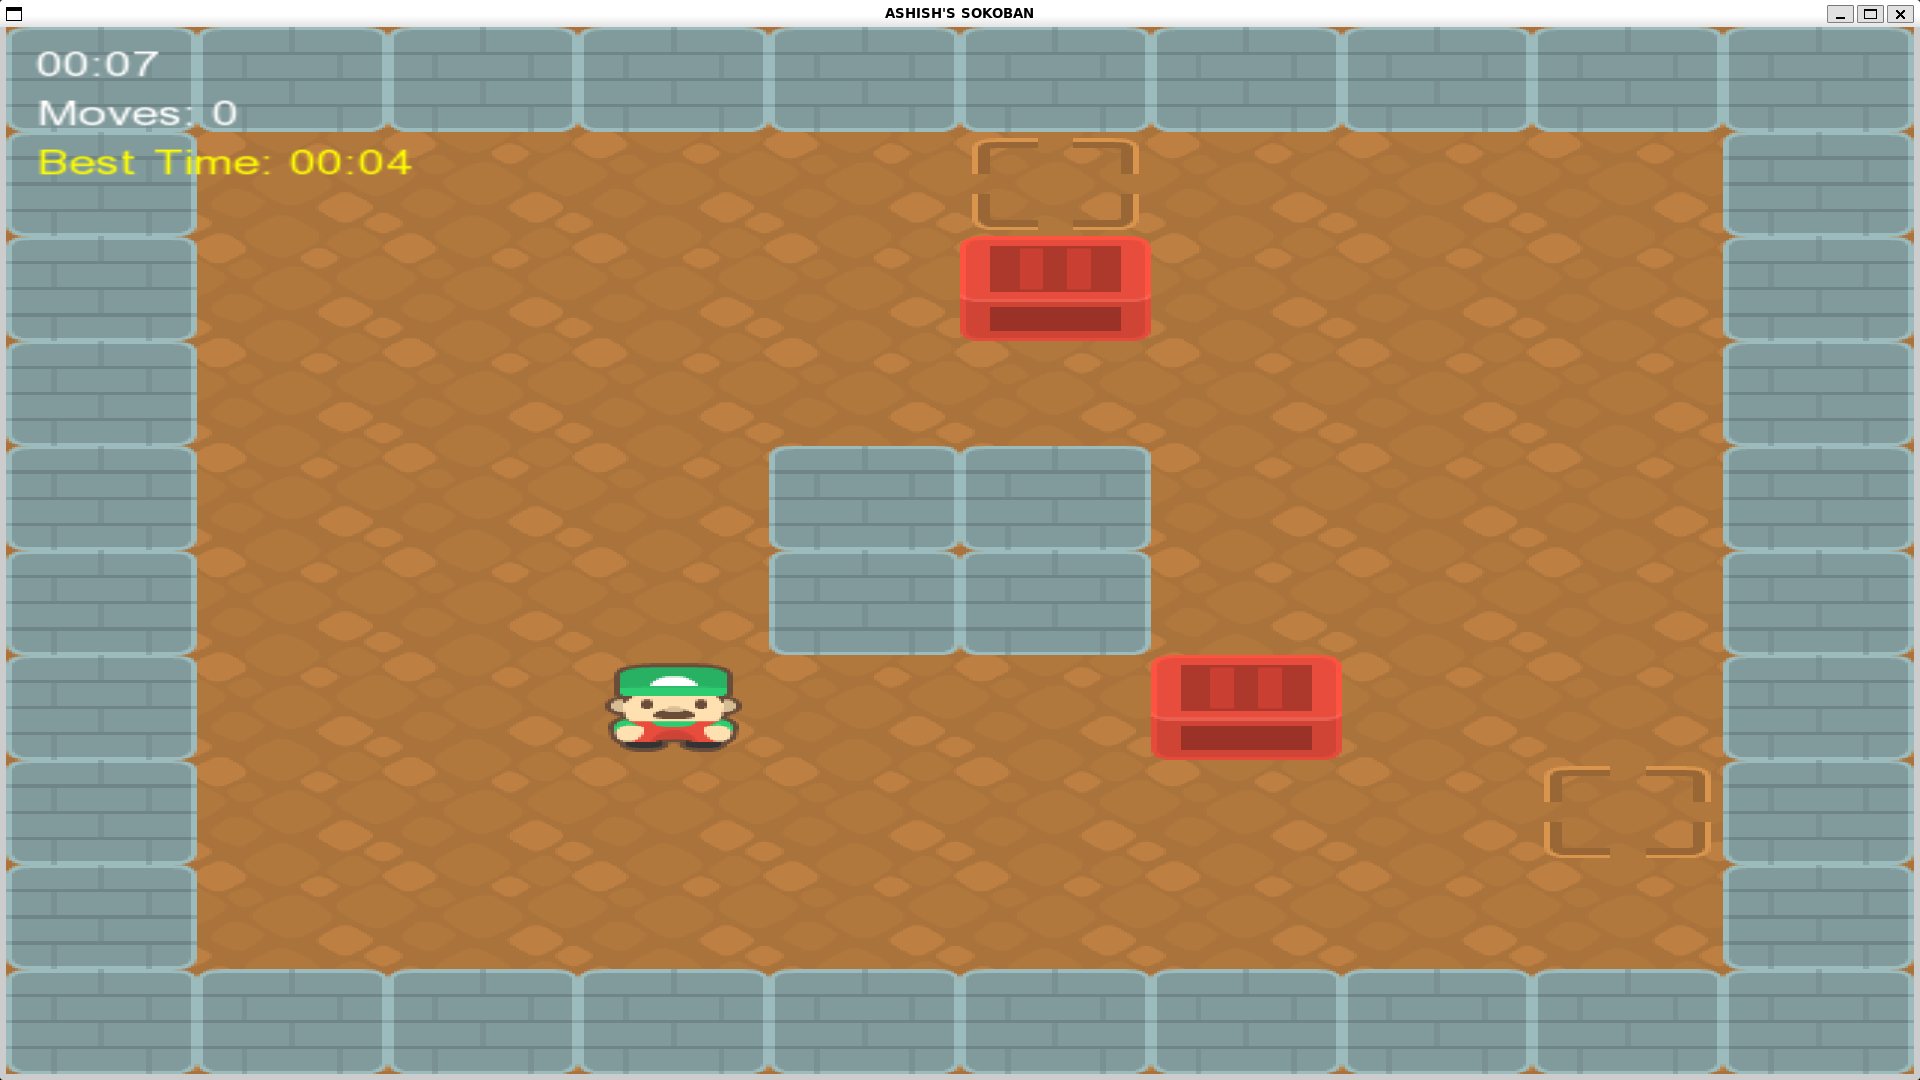
\includegraphics[width=10cm]{comp 4/images/ps4b_screenshot.png}
	\caption{My Sokoban}
\end{figure}
% PS4: Sokoban UI \& Sokoban
\newpage
\section{PS5: DNA Alignment}
\subsection{Overview}
I have implemented a program for DNA alignment, which aligns two given DNA sequences using a sequence alignment algorithm. The program computes the optimal alignment and displays the results. This project helped me understand the complexities of sequence alignment algorithms, which are fundamental in bioinformatics for comparing genetic sequences.
\subsection{What I Accomplished}
1. I have implemented an algorithm for aligning two DNA sequences, ensuring accurate matching of bases.
\newline
2. I have incorporated dynamic programming to compute the optimal alignment, including gaps and mismatches.

\subsection{What I Learned}
==$>$I understood how DNA alignment is used in real-world applications, such as genetic comparison and evolutionary studies.
\newline
==$>$I learned how sequence alignment algorithms work, including the concepts of scoring matrices, gaps, and penalties.
\newline
==$>$I understood how DNA alignment is used in real-world applications, such as genetic comparison and evolutionary studies.
\subsection{Discussion of Key Algorithms}
\textbf{Data Structures:}
\newline
1.2D Matrix:
\newline
==$>$Used to store the scoring values during the dynamic programming process for sequence alignment.
\newline
2. Vectors/Strings:
\newline 
==$>$Used to store the input DNA sequences and their aligned counterparts
\newline 
\textbf{Algorithms:}
\newline
1.Edit Distance:
\newline 
==$>$Matrix Initialization: The dynamic programming matrix (opt) is initialized with dimensions based on the lengths of the input strings x and y. The matrix is filled with zeros initially.
\newline
==$>$Filling the Matrix: The matrix is filled row by row using a recurrence relation
\newline
2.Dynamic Programming:
\newline
==$>$The matrix is filled based on recurrence relations, considering scores for matches, mismatches, and gap penalties.
\newline
3. Backtracking: 
\newline
==$>$Once the optimal matrix is built, backtracking is used to extract the aligned sequences.
\newline
\textbf{Object Oriented Designs:}
\newline
==$>$class:
\newline
The EDistance class played a vital role in this project for calculating the distances.
\newline
==$>$Exception Handling:
\newline
I have used exception handling to ensure that the input strings are valid or not.
\subsection{What I Already Knew}
1. String Manipulation:
\newline 
I had basic idea about string operations, which were crucial for handling and comparing DNA sequences in this project.
\newline
2. 2D Arrays/Matrix Handling:
\newline
I was familiar with using 2D arrays to store and manipulate data, which is important for the dynamic programming matrix in the alignment algorithm.
\subsection{Challenges}
==$>$I have faced difficulty in Ensuring that the algorithm handles various edge cases, such as empty strings, strings with one character, or strings with different lengths.
\newline
==$>$I have faced difficulty in the backtracking process to extract the optimal alignment
\subsection{Codes}
\subsubsection{Makefile}
\begin{lstlisting}[style=cppcode]
CXX = g++
CXXFLAGS = -std=c++20 -Wall -Werror -pedantic -g
LDFLAGS = -lsfml-system -lsfml-window -lsfml-graphics

all: EDistance test EDistance.a

EDistance: main.o EDistance.o
	$(CXX) $(CXXFLAGS) -o EDistance main.o EDistance.o $(LDFLAGS)

test: test.o EDistance.o
	$(CXX) $(CXXFLAGS) -o test test.o EDistance.o $(LDFLAGS) -lboost_unit_test_framework


EDistance.a: EDistance.o
	ar rcs EDistance.a EDistance.o

EDistance.o: EDistance.cpp EDistance.hpp
	$(CXX) $(CXXFLAGS) -c EDistance.cpp

main.o: main.cpp EDistance.hpp
	$(CXX) $(CXXFLAGS) -c main.cpp

test.o: test.cpp EDistance.hpp
	$(CXX) $(CXXFLAGS) -c test.cpp

lint:
	cppcheck --enable=all --std=c++11 .

clean:
	rm -f *.o EDistance test EDistance.a
\end{lstlisting}
\subsubsection{main.cpp}
\begin{lstlisting}[style=cppcode]
// Copyright Ashish Kosana [2024]
#include <iostream>
#include <iomanip>  // For std::setprecision
#include <cstdlib>  // For system calls to get memory usage
#include <cstring>
#include "EDistance.hpp"
#include <SFML/System.hpp>

// Function to get current memory usage (in MB)
double getMemoryUsageMB() {
    double memoryUsage = 0.0;
    FILE* file = fopen("/proc/self/status", "r");
    if (file) {
        char line[128];
        while (fgets(line, 128, file) != NULL) {
            if (strncmp(line, "VmRSS:", 6) == 0) {
                memoryUsage = strtod(line + 6, NULL) / 1024.0;  // Convert KB to MB
                break;
            }
        }
        fclose(file);
    }
    return memoryUsage;
}

int main() {
    std::string x, y;
    std::cin >> x >> y;

    double initialMemory = getMemoryUsageMB();

    sf::Clock clock;
    EDistance ed(x, y);
    int distance = ed.optDistance();
    std::cout << "Edit distance = " << distance << std::endl;
    std::cout << ed.alignment();

    // Print memory usage in MB
    double finalMemory = getMemoryUsageMB();
    double memoryUsedMB = finalMemory - initialMemory;
    std::cout << "Memory used: " << std::fixed << std::setprecision(2)
              << memoryUsedMB << " MB" << std::endl;

    // Print edit distance again after the sequence
    std::cout << "Edit distance after sequence = " << distance << std::endl;

    sf::Time elapsed = clock.getElapsedTime();
    std::cout << "Execution time is " << std::fixed << std::setprecision(6)
              << elapsed.asSeconds() << " seconds" << std::endl;
    return 0;
}

\end{lstlisting}
\subsubsection{EDistance.hpp}
\begin{lstlisting}[style=cppcode]
// Copyright Ashish Kosana [2024]
#ifndef EDISTANCE_HPP
#define EDISTANCE_HPP

#include <string>
#include <vector>

class EDistance {
 public:
    EDistance(const std::string& x, const std::string& y);
    static int penalty(char a, char b);
    static int min3(int a, int b, int c);
    int optDistance();
    std::string alignment();

 private:
    std::string x, y;
    std::vector<std::vector<int>> opt;
    void calculateOptDistance();
};

#endif  // EDISTANCE_HPP
\end{lstlisting}
\newpage
\subsubsection{EDistance.cpp}
\begin{lstlisting}[style=cppcode]

// Copyright Ashish Kosana [2024]
#include "EDistance.hpp"
#include <algorithm>
#include <stdexcept>

EDistance::EDistance(const std::string& x, const std::string& y) : x(x), y(y) {
    if (x.empty() || y.empty()) {
        throw std::invalid_argument("Input strings must not be empty.");
    }
    opt.resize(x.size() + 1, std::vector<int>(y.size() + 1, 0));
}

int EDistance::penalty(char a, char b) {
    return (a == b) ? 0 : 1;
}

int EDistance::min3(int a, int b, int c) {
    return std::min({a, b, c});
}

void EDistance::calculateOptDistance() {
    for (size_t i = 0; i <= x.size(); ++i)
        opt[i][y.size()] = 2 * (x.size() - i);

    for (size_t j = 0; j <= y.size(); ++j)
        opt[x.size()][j] = 2 * (y.size() - j);

    for (int i = x.size() - 1; i >= 0; --i) {
        for (int j = y.size() - 1; j >= 0; --j) {
            int matchOrMismatch = opt[i + 1][j + 1] + penalty(x[i], y[j]);
            int gapInX = opt[i + 1][j] + 2;
            int gapInY = opt[i][j + 1] + 2;
            opt[i][j] = min3(matchOrMismatch, gapInX, gapInY);
        }
    }
}

int EDistance::optDistance() {
    calculateOptDistance();
    return opt[0][0];
}

std::string EDistance::alignment() {
    std::string result;
    std::string::size_type i = 0;
    std::string::size_type j = 0;

    while (i < x.size() || j < y.size()) {
        // Check bounds before accessing opt[i][j]
        if (i < x.size() && j < y.size() &&
            opt[i][j] == opt[i + 1][j + 1] + penalty(x[i], y[j])) {
            // Align characters from both strings
            result += x[i] + std::string(" ") + y[j] + " " +
                      std::to_string(penalty(x[i], y[j])) + "\n";
            i++;
            j++;
        } else if (i < x.size() && (j == y.size() ||
                   opt[i][j] == opt[i + 1][j] + 2)) {
            // Align character from x with a gap in y
            result += x[i] + std::string(" - 2\n");
            i++;
        } else if (j < y.size()) {
            // Align character from y with a gap in x
            result += "- " + std::string(1, y[j]) + " 2\n";
            j++;
        }
    }

    return result;
}

\end{lstlisting}

\subsubsection{test.cpp}
\begin{lstlisting}[style=cppcode]
\texttt{ 
// Copyright Ashish Kosana [2024]
#include <stdexcept>
#define BOOST_TEST_MODULE EDistanceTest
#include <boost/test/included/unit_test.hpp>
#include "EDistance.hpp"

BOOST_AUTO_TEST_CASE(penalty_test) {
    BOOST_CHECK_EQUAL(EDistance::penalty('A', 'A'), 0);
    BOOST_CHECK_EQUAL(EDistance::penalty('A', 'T'), 1);
    BOOST_CHECK_EQUAL(EDistance::penalty('G', 'G'), 0);
    BOOST_CHECK_EQUAL(EDistance::penalty('C', 'A'), 1);
}

BOOST_AUTO_TEST_CASE(min3_test) {
    BOOST_CHECK_EQUAL(EDistance::min3(1, 2, 3), 1);
    BOOST_CHECK_EQUAL(EDistance::min3(3, 2, 1), 1);
    BOOST_CHECK_EQUAL(EDistance::min3(3, 3, 3), 3);
    BOOST_CHECK_EQUAL(EDistance::min3(-1, 0, 1), -1);
}

BOOST_AUTO_TEST_CASE(opt_distance_test) {
    EDistance ed("AACAGTTACC", "TAAGGTCA");
    BOOST_CHECK_EQUAL(ed.optDistance(), 7);

    EDistance ed2("ACGT", "ACGT");
    BOOST_CHECK_EQUAL(ed2.optDistance(), 0);
}

BOOST_AUTO_TEST_CASE(alignment_test) {
    EDistance ed("AACAGTTACC", "TAAGGTCA");
    int distance = ed.optDistance();
    BOOST_CHECK_EQUAL(distance, 7);

    std::string result = ed.alignment();
    BOOST_CHECK(!result.empty());
}

BOOST_AUTO_TEST_CASE(exception_handling_test) {
    BOOST_REQUIRE_THROW(EDistance("", "TACG"), std::invalid_argument);
    BOOST_REQUIRE_THROW(EDistance("ACGT", ""), std::invalid_argument);

    BOOST_REQUIRE_NO_THROW(EDistance("ACGT", "TACG"));
    BOOST_REQUIRE_NO_THROW(EDistance("A", "G"));
}

BOOST_AUTO_TEST_CASE(complex_alignment_test) {
    EDistance ed("ACGTACGT", "TACG");
    int distance = ed.optDistance();
    BOOST_CHECK_EQUAL(distance, 8);

    std::string result = ed.alignment();
    BOOST_CHECK(!result.empty());
    BOOST_CHECK(result.find("2\n") != std::string::npos);
}
}
\end{lstlisting}
\newpage
\subsubsection{Input:}
\begin{lstlisting}[style=cppcode]
./EDistance < example10.txt
\end{lstlisting}
\subsubsection{Output:}
\begin{lstlisting}[style=cppcode]
Edit distance = 7
A T 1
A A 0
C - 2
A A 0
G G 0
T G 1
T T 0
A - 2
C C 0
C A 1
Memory used: 0.00 MB
Edit distance after sequence = 7
Execution time is 0.000202 seconds
\end{lstlisting}
%PS5: DNA Alignment
\newpage
\section{PS6:RandWriter}
\subsection{Overview}
In the RandWriter project, I implemented a program that generates random text files based on user-defined parameters such as the number of words, sentences, or paragraphs. The program uses random word selection to build sentences and paragraphs, and the user can specify the desired output file size
\subsection{What I Accomplished}
1.I have implemented random word selection from a dictionary to ensure the generated text is readable.
\newline
2. I have added functionality for users to specify the desired output file size, making the program versatile for different types of testing or data generation.
\newline
3. I have implemented a program that generates random text files based on user-defined parameters
\subsection{What I Learned}
==$>$I have learned how to generate random characters based on probabilities.
\newline
==$>$I have learned how to use dictionaries to store data like character frequencies and probabilities.
\subsection{Discussion of Key Algorithms \& Data Structures}
\textbf{Data Structures:}
\newline
1. std::string: Used to handle individual words, sentences, and paragraphs that are generated.
\newline
2.std::ofstream: Used for writing the generated text to a file.
\newline
3. std::vector: Holds the sentences or paragraphs to ensure the program can handle multiple levels of text structure.
\newline
\textbf{Algorithms:}
\newline
1. Random Word Selection: The program selects random words from the dictionary to form sentences. It ensures the randomness and diversity of the text generated.
\newline
2. File Output: The program writes the generated content to a text file with user-specified parameters, such as file size or number of words.
\newline
\textbf{Object Oriented Designs:}
\newline
==$>$Exception Handling:
\newline
I have used exceptions (e.g: std::invalid argument) to handle errors in a controlled manner.
\newline
==$>$Operator Overloading:
\newline
The operator<< is overloaded as a friend function for easy printing of RandWriter objects.
\subsection{What I Already knew}
==$>$ I have girp over c++ programming concepts such as file handling,classes and objects.
\subsection{Challenges}
==$>$I have faced difficulty in understanding the k-gram concept and how to use it for text generation.
\newline
==$>$I have faced difficulty in the process of computing the frequency of k-grams and their subsequent characters.
\newline
==$>$I have faced difficulty in handling the invalid inputs, such as when the k-gram does not exist or when the order is zero.
\subsection{Codes}

\subsubsection{Makefile}
\begin{lstlisting}[style=cppcode]
CXX = g++
CXXFLAGS = -std=c++17 -Wall -Wextra -pedantic -Werror
TEST_LIBS = -lboost_unit_test_framework

all: TextWriter test TextWriter.a

TextWriter: TextWriter.o RandWriter.o
	$(CXX) $(CXXFLAGS) -o $@ $^

TextWriter.a: RandWriter.o
	ar rcs $@ $^

test: test.o RandWriter.o
	$(CXX) $(CXXFLAGS) -o $@ $^ $(TEST_LIBS)

%.o: %.cpp
	$(CXX) $(CXXFLAGS) -c $<

lint:
	cpplint *.cpp *.hpp

clean:
	rm -f *.o TextWriter TextWriter.a test

.PHONY: all lint clean
\end{lstlisting}
\subsubsection{RandWriter.hpp}
\begin{lstlisting}[style=cppcode]
// Copyright [2024] Ashish Kosana

#include <string>
#include <unordered_map>
#include <unordered_set>
#include <vector>
#include <iostream>
#include <stdexcept>
#include <random>

class RandWriter {
 public:
    RandWriter(const std::string& input_text, size_t order);
    size_t orderK() const;

    int freq(const std::string& kgram) const;
    int freq(const std::string& kgram, char c) const;
    char kRand(const std::string& kgram);
    std::string generate(const std::string& kgram, size_t L);

    friend std::ostream& operator<<(std::ostream& os, const RandWriter& rw);

 private:
    void populateKgramMap();
    char weightedRandomChar(const std::unordered_map<char, int>& charFreq) const;

    size_t k;
    std::string text;
    std::unordered_map<std::string, std::unordered_map<char, int>> kgram_map;
};
\end{lstlisting}
\subsubsection{RandWriter.cpp}
\begin{lstlisting}[style=cppcode]
// Copyright [2024] Ashish Kosana
#include "RandWriter.hpp"
#include <iostream>
#include <stdexcept>
#include <unordered_map>
#include <unordered_set>
#include <vector>
#include <random>


thread_local std::mt19937 gen(std::random_device {}());

RandWriter::RandWriter(const std::string& input_text, size_t order)
    : k(order), text(input_text) {
    if (text.empty()) {
        throw std::invalid_argument("Input text cannot be empty");
    }
    if (k > text.size()) {
        throw std::invalid_argument("Order k cannot exceed input text length");
    }

    if (k > 0) {
        populateKgramMap();
    }
}

size_t RandWriter::orderK() const {
    return k;
}

void RandWriter::populateKgramMap() {
    size_t n = text.size();
    for (size_t i = 0; i < n; ++i) {
        std::string kgram = text.substr(i, k);

        // Wrap-around handling for k-grams
        if (kgram.size() < k) {
            kgram += text.substr(0, k - kgram.size());
        }

        char next_char = text[(i + k) % n];
        kgram_map[kgram][next_char]++;
    }
}

int RandWriter::freq(const std::string& kgram) const {
    if (k == 0) {
        if (kgram.empty()) {
            return text.size();
        }
        throw std::invalid_argument("kgram must be empty when k = 0");
    }
    if (kgram.size() != k) {
        throw std::invalid_argument("kgram must be of length k");
    }
    auto it = kgram_map.find(kgram);
    if (it == kgram_map.end()) {
        return 0;
    }
    int total = 0;
    for (const auto& pair : it->second) {
        total += pair.second;
    }
    return total;
}

int RandWriter::freq(const std::string& kgram, char c) const {
    if (k == 0) {
        return 0;  // No k-grams exist for k = 0
    }
    if (kgram.size() != k) {
        throw std::invalid_argument("kgram must be of length k");
    }
    auto it = kgram_map.find(kgram);
    if (it == kgram_map.end()) {
        return 0;
    }
    auto char_it = it->second.find(c);
    return (char_it != it->second.end()) ? char_it->second : 0;
}

char RandWriter::kRand(const std::string& kgram) {
    if (k == 0) {
        throw std::invalid_argument("kRand not valid for k = 0");
    }
    if (kgram.size() != k) {
        throw std::invalid_argument("kgram must be of length k");
    }
    auto it = kgram_map.find(kgram);
    if (it == kgram_map.end()) {
        throw std::invalid_argument("kgram not found in text");
    }
    return weightedRandomChar(it->second);
}

char RandWriter::weightedRandomChar(const std::unordered_map<char, int>& charFreq) const {
    std::vector<char> chars;
    std::vector<int> weights;

    for (const auto& pair : charFreq) {
        chars.push_back(pair.first);
        weights.push_back(pair.second);
    }

    std::discrete_distribution<> dist(weights.begin(), weights.end());
    return chars[dist(gen)];
}

std::string RandWriter::generate(const std::string& kgram, size_t L) {
    if (k == 0) {
        throw std::invalid_argument("Cannot generate text with k = 0");
    }
    if (kgram.size() != k) {
        throw std::invalid_argument("kgram must be of length k");
    }
    if (L < k) {
        throw std::invalid_argument("L must be at least k");
    }

    std::string result = kgram;
    for (size_t i = k; i < L; ++i) {
        char next_char = kRand(result.substr(result.size() - k, k));
        result += next_char;
    }
    return result;
}

std::ostream& operator<<(std::ostream& os, const RandWriter& rw) {
    os << "Order: " << rw.k << "\nAlphabet: ";
    std::unordered_set<char> alphabet;
    for (char c : rw.text) {
        alphabet.insert(c);
    }
    for (char c : alphabet) {
        os << c << " ";
    }
    os << "\nFrequencies:\n";
    for (const auto& pair : rw.kgram_map) {
        os << pair.first << ": ";
        for (const auto& sub_pair : pair.second) {
            os << sub_pair.first << "(" << sub_pair.second << ") ";
        }
        os << "\n";
    }
    return os;
}

\end{lstlisting}
\subsubsection{TextWriter.cpp}
\begin{lstlisting}[style=cppcode]
// Copyright [2024] Ashish Kosana
#include <iostream>
#include <fstream>
#include <stdexcept>
#include "RandWriter.hpp"

int main(int argc, char* argv[]) {
    if (argc != 3) {
        std::cerr << "Usage: ./TextWriter <order> <length>\n";
        return 1;
    }

    size_t k = 0, L = 0;
    try {
        k = std::stoi(argv[1]);
        L = std::stoi(argv[2]);
    } catch (const std::exception& e) {
        std::cerr << "Error parsing arguments: " << e.what() << std::endl;
        return 1;
    }

    std::string text((std::istreambuf_iterator<char>(std::cin)),
                     std::istreambuf_iterator<char>());

    if (text.empty()) {
        std::cerr << "Error: No input text provided.\n";
        return 1;
    }

    try {
        RandWriter writer(text, k);


        auto generateKgram = [&text, k]() { return text.substr(0, k); };

        std::string kgram = generateKgram();
        std::cout << writer.generate(kgram, L) << std::endl;
    } catch (const std::exception& e) {
        std::cerr << "Error: " << e.what() << std::endl;
        return 1;
    }

    return 0;
}
\end{lstlisting}

\subsubsection{test.cpp}
\begin{lstlisting}[style=cppcode]
// Copyright [2024] Ashish Kosana

#define BOOST_TEST_MODULE RandWriterTests
#define BOOST_TEST_DYN_LINK
#include <stdexcept>
#include <boost/test/unit_test.hpp>
#include "RandWriter.hpp"

BOOST_AUTO_TEST_CASE(TestConstructor) {
    // Test valid construction
    BOOST_REQUIRE_NO_THROW(RandWriter("abcde", 2));
    BOOST_REQUIRE_NO_THROW(RandWriter("abc", 0));

    // Test invalid construction
    BOOST_REQUIRE_THROW(RandWriter("", 2), std::invalid_argument);
    BOOST_REQUIRE_THROW(RandWriter("abc", 4), std::invalid_argument);
}

BOOST_AUTO_TEST_CASE(TestOrderK) {
    RandWriter rw("abcde", 2);
    BOOST_REQUIRE_EQUAL(rw.orderK(), 2);
}

BOOST_AUTO_TEST_CASE(TestFreq) {
    RandWriter rw("abcabcabc", 2);
    BOOST_REQUIRE_EQUAL(rw.freq("ab"), 3);
    BOOST_REQUIRE_EQUAL(rw.freq("bc"), 3);
    BOOST_REQUIRE_EQUAL(rw.freq("ca"), 3);
    BOOST_REQUIRE_EQUAL(rw.freq("ab", 'c'), 3);
    BOOST_REQUIRE_THROW(rw.freq("a"), std::invalid_argument);
    BOOST_REQUIRE_THROW(rw.freq("abc"), std::invalid_argument);
}

BOOST_AUTO_TEST_CASE(TestKRand) {
    RandWriter rw("abcabcabc", 2);
    BOOST_REQUIRE_NO_THROW(rw.kRand("ab"));
    BOOST_REQUIRE_THROW(rw.kRand("xy"), std::invalid_argument);
    BOOST_REQUIRE_THROW(rw.kRand("a"), std::invalid_argument);
}

BOOST_AUTO_TEST_CASE(TestGenerate) {
    RandWriter rw("abcabcabc", 2);
    std::string generated = rw.generate("ab", 10);
    BOOST_REQUIRE_EQUAL(generated.length(), 10);
    BOOST_REQUIRE_EQUAL(generated.substr(0, 2), "ab");
    BOOST_REQUIRE_THROW(rw.generate("ab", 1), std::invalid_argument);
    BOOST_REQUIRE_THROW(rw.generate("a", 5), std::invalid_argument);
}

\end{lstlisting}
\subsubsection{Input:}
\begin{lstlisting}[style=cppcode]
./TextWriter 2 11 <  input17.txt
\end{lstlisting}
\subsubsection{Output:}
\begin{lstlisting}[style=cppcode]
gaggaagagag
\end{lstlisting}
%PS6:RandWriter
\newpage
\section{PS7: Kronos Log Parsing}
\subsection{Overview}
In this project, I have implemented a program to parse and analyze log files from the Kronos InTouch device, which is a Linux-based touch-screen time clock. The main aim is to identify device startup sequences, and  determine whether they were successful or incomplete, and calculate the duration of each boot process
\subsection{What I Accomplished}
1. I have implemented a program in C++ to parse Kronos InTouch logs and analyze boot-up data.
\newline
2. I have used regular expressions to identify boot start and completion events.
\newline
3. I have calculated boot durations using timestamps and the Boost Date-Time library.
\newline
4. I have  handled edge cases like incomplete or nested boot sequences and ensured these were included in the final report.
\newline
5. I have generated structured output reports that summarized key boot details.
\subsection{What I Learned}
1. I have learned how to analyze and process real-world log files to extract meaningful insights.
\newline
2. I have improved my understanding of regular expressions and their application in parsing structured text.
\newline
3. I have also gained the experience using the Boost Date-Time library for precise time calculations.
\subsection{Discussion of Key Algorithms}
\textbf{Data Structures:}
\newline
1. \texttt{std::vector<std::pair<std::string, std::string>>}
\newline
To store matched log entries as pairs of timestamps and event types ("Boot Start" or "Boot Complete").
\newline
2. \texttt{std::unordered\_map<int, std::vector<std::string>>}
\newline
It is used for associating sequence IDs with corresponding log events, facilitating organized and efficient data retrieval.
\newline
3. std::tm 
\newline
It is used for parsing and storing timestamp details extracted from log entries.
\newline
4. std::regex
\newline
It is used for defining and matching patterns in the log data to identify relevant events
\newline
\textbf{Algorithms:}
\newline
1. Log Parsing
\newline
I have implemented a regular expression-based on the approach to match specific patterns in log entries.
\newline
2. Output Formatting
\newline
==$>$I have formatted the final output into a structured report with clear sections:
\newline
i.) Boot sequence ID.
\newline
ii.) Start and completion timestamps.
\newline
iii.) Boot duration in milliseconds.
\newline
iv.) Incomplete boots were categorized in a separate section for clarity.
\newline
\textbf{Object Oriented Designs:}
\newline
==$>$Class:
The BootRecord class is the key part of the project, as it encapsulates all the  details about each boot event.
\newline
==$>$Encapsulation:
\newline 
The BootRecord class encapsulates all the data for each boot event.
\subsection{What I Already Knew}
==$>$I was already familiar with some basic file handling operations in C++ for reading and writing data.
\subsection{Challenges}
==$>$I have faced difficulty in Processing large log files efficiently.
\newline
==$>$I have faced difficulty in Parsing timestamps and calculating durations accurately .
\newline
==$>$I have faced difficulty in identifying and processing logs for incomplete boots .
\subsection{Codes}

\subsubsection{Makefile}
\begin{lstlisting}[style=cppcode]

# Compiler and flags
CXX = g++
CXXFLAGS = -std=c++17 -Wall -Wextra -Werror -O2 -pedantic

# Targets
SRC = ps7.cpp
OBJ = $(SRC:.cpp=.o)
EXE = ps7

# Default target
all: $(EXE)

# Build the executable
$(EXE): $(OBJ)
	$(CXX) $(CXXFLAGS) -o $@ $^

# Compile object files
%.o: %.cpp
	$(CXX) $(CXXFLAGS) -c $< -o $@

# Linting (optional, use a tool like clang-tidy if available)
lint:
	clang-tidy $(SRC)

# Clean up generated files
clean:
	rm -f $(OBJ) $(EXE) *.rpt
\end{lstlisting}

\subsubsection{ps7.cpp}
\begin{lstlisting}[style=cppcode]
// Copyright [2024] Ashish Kosana
#include <iostream>
#include <fstream>
#include <regex>
#include <string>
#include <vector>
#include <chrono>
#include <iomanip>
#include <sstream>

struct BootRecord {
    int startLine;
    int endLine;
    std::string startTime;
    std::string endTime;
    bool completed;
    int durationMs;
};

std::regex startRegex(R"(\(log\.c\.166\) server started)");
std::regex endRegex(R"(oejs\.AbstractConnector:Started .+)");

int calculateDurationMs(const std::string& start, const std::string& end) {
    std::tm tmStart = {}, tmEnd = {};
    std::istringstream ssStart(start);
    std::istringstream ssEnd(end);
    ssStart >> std::get_time(&tmStart, "%Y-%m-%d %H:%M:%S");
    ssEnd >> std::get_time(&tmEnd, "%Y-%m-%d %H:%M:%S");

    auto startTime = std::chrono::
    system_clock::from_time_t(std::mktime(&tmStart));
    auto endTime = std::chrono::
    system_clock::from_time_t(std::mktime(&tmEnd));
    return std::chrono::duration_cast<std::chrono::milliseconds>(
        endTime - startTime).count();
}

std::vector<BootRecord> parseLogFile(const std::string& filename) {
    std::vector<BootRecord> bootRecords;
    std::ifstream file(filename);
    std::string line;
    int lineNumber = 0;
    BootRecord currentBoot;
    bool inBoot = false;

    if (!file.is_open()) {
        std::cerr << "Error: Unable to open file " << filename << std::endl;
        return bootRecords;
    }

    while (std::getline(file, line)) {
        lineNumber++;
        std::smatch match;

        if (std::regex_search(line, match, startRegex)) {
            if (inBoot) {
                currentBoot.completed = false;
                bootRecords.push_back(currentBoot);
            }
            inBoot = true;
            currentBoot = BootRecord{lineNumber, 0,
            line.substr(0, 19), "", false, 0};
        } else if (inBoot && std::regex_search(line, match, endRegex)) {
            currentBoot.endLine = lineNumber;
            currentBoot.endTime = line.substr(0, 19);
            currentBoot.completed = true;
            currentBoot.durationMs = calculateDurationMs(
            currentBoot.startTime, currentBoot.endTime);
            bootRecords.push_back(currentBoot);
            inBoot = false;
        }
    }

    if (inBoot) {
        currentBoot.completed = false;
        bootRecords.push_back(currentBoot);
    }

    file.close();
    return bootRecords;
}

void generateReport(const std::string&
inputFile, const std::string& outputFile,
                    const std::vector<BootRecord>& bootRecords) {
    std::ofstream out(outputFile);
    if (!out.is_open()) {
        std::cerr << "Error: Unable to create output file "
        << outputFile << std::endl;
        return;
    }

    out << "Device Boot Report" << std::endl;
    out << "InTouch log file: " << inputFile << std::endl;
    out << "Summary:" << std::endl << std::endl;

    for (const auto& record : bootRecords) {
        out << "Device Boot - " << std::endl;
        out << record.startLine << "(" << inputFile << "): " << record.startTime
            << " Boot Start" << std::endl;
        if (record.completed) {
            out << record.endLine << "(" << inputFile << "): " << record.endTime
                << " Boot Completed\t   Time: " << record.durationMs << "ms"
                << std::endl;
        } else {
            out << "Boot Incomplete" << std::endl;
        }
        out << std::endl;
    }

    out.close();
    std::cout << "Report generated successfully in: "
    << outputFile << std::endl;
}

std::vector<std::string> getEndTimes(
    const std::vector<BootRecord>& records) {
    std::vector<std::string> endTimes;
    for (const auto& record : records) {
        if (!record.completed) {
            endTimes.push_back(record.startTime);
        }
    }
    return endTimes;
}

int main(int argc, char* argv[]) {
    if (argc != 2) {
        std::cerr << "Usage: " << argv[0] << " <logfile>" << std::endl;
        return 1;
    }

    std::string inputFile = argv[1];
    std::string outputFile = inputFile + ".rpt";

    auto bootRecords = parseLogFile(inputFile);
    generateReport(inputFile, outputFile, bootRecords);

    auto failedBoots = getEndTimes(bootRecords);
    std::cout << "Failed Boots: " << failedBoots.size() << std::endl;
    for (const auto& time : failedBoots) {
        std::cout << time << std::endl;
    }

    return 0;
}

\end{lstlisting}
\subsubsection{Output:}
\begin{lstlisting}[style=cppcode]
Device Boot Report
InTouch log file: device1_intouch.log
Summary:

Device Boot - 
435369(device1_intouch.log): 2014-03-25 19:11:59 Boot Start
435759(device1_intouch.log): 2014-03-25 19:15:02 Boot Completed	   Time: 183000ms

Device Boot - 
436500(device1_intouch.log): 2014-03-25 19:29:59 Boot Start
436859(device1_intouch.log): 2014-03-25 19:32:44 Boot Completed	   Time: 165000ms

Device Boot - 
440719(device1_intouch.log): 2014-03-25 22:01:46 Boot Start
440791(device1_intouch.log): 2014-03-25 22:04:27 Boot Completed	   Time: 161000ms

Device Boot - 
440866(device1_intouch.log): 2014-03-26 12:47:42 Boot Start
441216(device1_intouch.log): 2014-03-26 12:50:29 Boot Completed	   Time: 167000ms

Device Boot - 
442094(device1_intouch.log): 2014-03-26 20:41:34 Boot Start
442432(device1_intouch.log): 2014-03-26 20:44:13 Boot Completed	   Time: 159000ms

Device Boot - 
443073(device1_intouch.log): 2014-03-27 14:09:01 Boot Start
443411(device1_intouch.log): 2014-03-27 14:11:42 Boot Completed	   Time: 161000ms

\end{lstlisting}
%PS7: Kronos Log Parsing
\end{document}
